% \documentclass[anon,12pt]{colt2018} % Anonymized submission
\documentclass[final]{colt2018} % Include author names

% The following packages will be automatically loaded:
% amsmath, amssymb, natbib, graphicx, url, algorithm2e

\usepackage[utf8]{inputenc} % allow utf-8 input
\usepackage[T1]{fontenc}    % use 8-bit T1 fonts
\usepackage{hyperref}       % hyperlinks
\usepackage{url}            % simple URL typesetting
\usepackage{booktabs}       % professional-quality tables
\usepackage{amsfonts}       % blackboard math symbols
\usepackage{nicefrac}       % compact symbols for 1/2, etc.
\usepackage{microtype}      % microtypography
\usepackage{transparent}

% \usepackage{amsmath}
%\usepackage{amsthm}
% \usepackage{amssymb}
\usepackage{mathtools}
%\usepackage[usenames]{xcolor}

%\usepackage[ruled,linesnumbered]{algorithm2e}

\usepackage{enumitem}
\setitemize{noitemsep,topsep=0pt,parsep=0pt,partopsep=0pt}

\definecolor{darkblue}{rgb}{0.0,0.0,0.55}
\hypersetup{
	colorlinks = true,
	citecolor  = darkblue,
	linkcolor  = darkblue,
	citecolor  = darkblue,
	filecolor  = darkblue,
	urlcolor   = darkblue,
}


\usepackage{enumitem}
\usepackage{xspace}

\usepackage{wrapfig}

%\newtheorem{lemma}{Lemma}
%\newtheorem{theorem}{Theorem}
%\newtheorem{corollary}{Corollary}
%\newtheorem{proposition}{Proposition}
%\newtheorem{remark}{Remark}
%\newtheorem{definition}{Definition}
\newtheorem{claim}{Claim}
\newtheorem{assumption}{Assumption}

\newcommand{\Exp}{\mathrm{Exp}}
\newcommand{\arccosh}{\mathrm{arccosh}}
\newcommand\numberthis{\addtocounter{equation}{1}\tag{\theequation}}
\newcommand{\ragd}{\textsc{Ragd}}
\newcommand{\inj}{\mathrm{inj}}
\renewcommand{\nabla}{\mathrm{grad}}

\title[An Estimate Sequence for Geodesically Convex Optimization]{An Estimate Sequence for Geodesically Convex Optimization}
\usepackage{times}
 % Use \Name{Author Name} to specify the name.
 % If the surname contains spaces, enclose the surname
 % in braces, e.g. \Name{John {Smith Jones}} similarly
 % if the name has a "von" part, e.g \Name{Jane {de Winter}}.
 % If the first letter in the forenames is a diacritic
 % enclose the diacritic in braces, e.g. \Name{{\'E}louise Smith}

 % Two authors with the same address
  % \coltauthor{\Name{Author Name1} \Email{abc@sample.com}\and
  %  \Name{Author Name2} \Email{xyz@sample.com}\\
  %  \addr Address}

 % Three or more authors with the same address:
 % \coltauthor{\Name{Author Name1} \Email{an1@sample.com}\\
 %  \Name{Author Name2} \Email{an2@sample.com}\\
 %  \Name{Author Name3} \Email{an3@sample.com}\\
 %  \addr Address}


 % Authors with different addresses:
 \coltauthor{\Name{Hongyi Zhang} \Email{hongyiz@mit.edu}\\
 \addr BCS and LIDS, Massachusetts Institute of Technology
 \AND
 \Name{Suvrit Sra} \Email{suvrit@mit.edu}\\
 \addr EECS and LIDS, Massachusetts Institute of Technology
 }

\begin{document}

\maketitle

\begin{abstract}
We propose a Riemannian version of Nesterov's Accelerated Gradient algorithm (\ragd), and show that for \emph{geodesically} smooth and strongly convex problems, within a neighborhood of the minimizer whose radius depends on the condition number as well as the sectional curvature of the manifold, \ragd{} converges to the minimizer with acceleration. Unlike the algorithm in \citep{liu2017accelerated} that requires the exact solution to a nonlinear equation which in turn may be intractable, our algorithm is constructive and computationally tractable\footnote{ as long as Riemannian gradient, exponential map and its inverse are computationally tractable, which is the case for many matrix manifolds \citep{absil2009optimization}.}. Our proof exploits a new estimate sequence and a novel bound on the nonlinear metric distortion, both ideas may be of independent interest.
\end{abstract}

\begin{keywords}
	Riemannian optimization; geodesically convex optimization; Nesterov's accelerated gradient method; nonlinear optimization
\end{keywords}

% !TeX root = main.tex
\section{Introduction}
\label{sec:intro}
Generative models are often trained in an unsupervised fashion, fitting a model $q$ to a set of observed data $x_P \subseteq X$ drawn iid from some true distribution $p$ on $x\in X$. Now, of course $p$ may not exactly belong to family $Q$ of probability distributions being fit, whether $Q$ consists of Gaussians mixture models, Markov models, or even neural networks of bounded size. We first discuss the limitations of generative modeling without feedback, and then discuss our model and results.

%\subsection{Limitations of Generative Modeling from Positive Examples Alone}
Consider fitting a generative model on a text corpus consisting partly of poetry written by four-year-olds and partly of mathematical publications from the {\em Annals of Mathematics}. Suppose that learning to generate a poem that looks like it was written by a child was easier than learning to generate a novel mathematical article with a correct, nontrivial statement. If the generative model pays a high price for generating unrealistic examples, then it may be better off learning to generate children's poetry than mathematical publications. However, without negative feedback, it may be difficult for a neural network or any other model to know that the mathematical articles it is generating are stylistically similar to the mathematical publications but do not contain valid proofs.\footnote{This is excluding clearly fake articles published without proper review in lower-tier venues \citep{LabbeL13}.} 

As a simpler example, the classic Markovian ``trigram model'' of natural language assigns each word a fixed probability conditioned only on the previous two words. Prior to recent advances in deep learning, for decades the trigram model and its variant were the workhorses of language modeling, assigning much greater likelihood to natural language corpora than numerous linguistically motivated grammars and other attempts \citep{Rosenfeld00}. However, text sampled from a trigram is typically nonsensical, e.g., the following text was randomly generated from a trigram model fit on a corpus of text from the Wall Street Journal \citep{JurafskyM09}:
\begin{quote}
They also point to ninety nine point six billion dollars from two hundred
four oh six three percent of the rates of interest stores as Mexico and
gram Brazil on market conditions. 
\end{quote}

In some applications, like text compression using a language model \citep{WittenNC87}, maximizing likelihood is equivalent to optimizing compression. However, in many  applications involving generation, such nonsense is costly and unacceptable. Now, of course it is possible to always generate valid data by returning random training examples, but this is simply overfitting and not learning. Alternatively, one could incorporate human-in-the-loop feedback such as through crowdsourcing, into the generative model to determine what is a valid, plausible sentence.

In some domains, validity could be determined automatically. Consider a Markovian model of a well-defined concept such as mathematical formulas that compile in \LaTeX{}. Now, consider a $n$-gram Markovian character model which the probability of each subsequent character is determined by the previous $n$ characters. For instance, the expression \$\{2+\{x-y\}\$ is invalid in \LaTeX{} due to mismatched braces. For this problem, a \LaTeX{} compiler may serve as a validity oracle. Various $n$-gram models can be fit which only generate valid formulas. To address mismatched braces, for example, one such model would ensure that it always closed braces within $n$ characters of opening, and had no nested braces. While an $n$-gram model will not perfectly model the true distribution over valid \LaTeX{} formulas, for certain generative purposes one may prefer an $n$-gram model that generates valid formulas over one that assigns greater likelihood to the training data but generates invalid formulas. 

Figure \ref{fig:rectangle} illustrates a simple case of learning a rectangle model for data which is not uniform over a rectangle. A maximum likelihood model would necessarily be the smallest rectangle containing all the data, but most examples generated from this distribution may be invalid. Instead a smaller rectangle, as illustrated in the figure, may be desired.

\begin{figure}[h]\label{fig:rectangle}
\centering
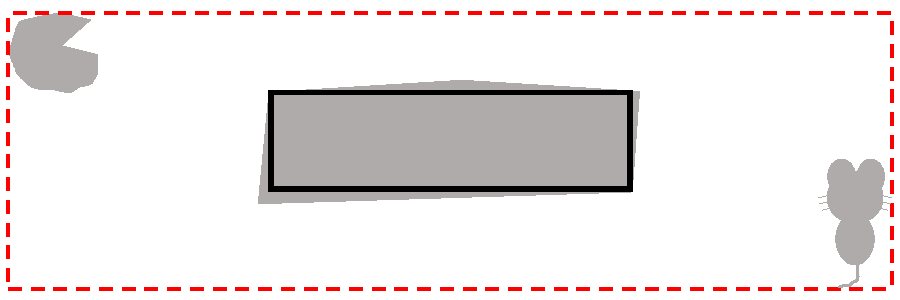
\includegraphics[width=3in]{fig.pdf}
\caption{Example where the underlying distribution $p$ is uniform over the (gray) valid regions. The solid rectangle maximizes our objective since it does not output nonsense (is supported only within the grey matter) and is closest to the $p$ (covers the maximum amount of grey matter). In contrast, the standard maximum likelihood (dashed red) rectangle must fully contain the observed samples, thus generating invalid points most of the time.  }
\end{figure}

Motivated by these observations, we evaluate a generative model $q$ on two axes. First is {\em coverage}, which is related to the probability assigned to future examples drawn from the true distribution $p$. Second is {\em validity}, defined as the probability that random examples generated from $q$ meet some validity requirement. Formally, we measure coverage in terms of a bounded {\em loss}:
$$\Loss(p,q)=\E_{x \sim p}[L(q_x)],$$
where $L:[0,1]\rightarrow [0,M]$ is a bounded decreasing function such as the capped log-loss $L(q_x)=\min(M, \log 1/q_x)$. % or $L(q_x)=\log 1/(q_x+\exp(-M))$. 
A bounded loss has the advantages of being efficiently estimable, and also it enables a model to assign 0 probability to one example (e.g., an outlier or error) if it greatly increases the likelihood of all other data. Validity is defined with respect to a set $V \subseteq X$, and $q(V)$ is the probability that a random example generated from $q$ lies within $V$. 

Clearly, there is a tradeoff between coverage and validity. We first focus on the case of (near) perfect validity. A Valid Generative Modeling (VGM) algorithm if it outputs, for a family of distributions $Q$ over $X$, if it outputs $\hat{q}$ with (nearly) perfect validity and whose loss is nearly as good as the loss of the best valid $q\in Q$. More precisely, $A$ is a VGM learner of $Q$ if for any nonempty valid subset $V \subseteq X$, any probability distribution $p$ over $V$, and any $\eps>0$, $A$ uses $n$ random samples from $p$ and makes $m$ membership oracle calls to $V$ and outputs a distribution $\hat{q}$ such that, $$\Loss(p, \hat{q}) \leq \min_{q \in Q: q(V)=1}\Loss(p,q) + \eps ~\text{ and }~\hat{q}(V)\geq 1-\eps.$$ 
We aim for our learner to be sample and query efficient, requiring that $n$ and $m$ are polynomial in $M, 1/\eps$ and a measure of complexity of our distribution class $Q$.
Furthermore, we would like our algorithms to be computationally efficient, with a runtime polynomial in the size of the data, namely the $n + m$ training examples. 
A more formal description of the problem is available in Section~\ref{sec:problem}.

$A$ is said to be {\em proper} if it always outputs $\hat{q}\in Q$ and {\em improper} otherwise.
In Section~\ref{sec:impossibility}, we first show that efficient proper learning for VGM is impossible. This is an information-theoretic result, meaning that even given infinite runtime and positive samples, one still cannot solve the VGM problem. Interestingly, this is different from binary classification, where it is possible to statistically learn from iid examples without a membership oracle.

Our first main positive result is an efficient (improper) learner for VGM. The algorithm relies on a subroutine that solves the following {\em Generative Modeling with Negatives} (GMN) problem: given sets $X_P, X_N \subset X$ of positive and negative examples, find the probability distribution $q \in Q$ which minimizes $\sum_{x \in X_P} L(q(x))$ subject to the constraint that $q(X_N)=0$. For simplicity, we present our algorithm for the case that the distribution family $Q$ is finite, giving sample and query complexity bounds that are logarithmic in terms of $|Q|$. However, as we show in Section~\ref{sec:infinite-families}, all of our results extend to infinite families $Q$. It follows that if one has a computationally efficient algorithm for the GMN problem for a distribution family $Q$, then our reduction gives a computationally efficient VGM learning algorithm for $Q$.

Our second positive result is an algorithm that minimizes $\Loss(p,q)$ subject to a relaxed validity constraint comparing against the optimal distribution that has validity $q(V)$ at least $1-\alpha$ for some $\alpha>0$. We show in Section~\ref{sec:partial-validity} that even in this more general setting, it is possible to obtain an algorithm that is statistically efficient but may not be computationally efficient. An important open question is whether there exists a computationally efficient algorithm for this problem when given access to an optimization oracle, as was the case for our algorithm for VGM.

\subsection{Related Work}
\cite{KearnsMRRSS94} showed how to learn distributions from positive examples in the realizable setting, i.e., where the true distribution is assumed to belong to the class being learned. In the same sense as their work is similar to PAC learning \citet{Valiant84} of distributions, our work is like agnostic learning \citet{KearnsSS94} in which no assumption on the true distribution is made. 

Generative Adversarial Networks (GANs)~\cite{GoodfellowPMXWOCB14} are an approach for generative modeling from positive examples alone, in which a generative model is trained against a discriminator that aims to distinguish real data from generated data. In some domains, GANs have been shown to outperform other methods at generating realistic-looking examples. Several shortcomings of GANs have been observed \citet{AroraRZ18}, and GANs are still subject to the theoretical limitations we argue are inherent to any model trained without a validity oracle. 

In supervised learning, there is a rich history of learning theory with various types of queries, including membership which are not unlike our (in)validity oracle. Under various assumptions, queries have been shown to facilitate the learning of complex classes such as finite automata \citet{Angluin88} and DNFs \citet{Jackson97}. See the survey of \cite{Angluin92} for further details.  Interestingly, \cite{Feldman09} has shown that for agnostic learning, i.e., without making assumptions on the generating distribution, the addition of membership queries does not enhance what is learnable beyond random examples alone. 
Supervised learning also has a large literature around active learning, showing how the ability to query examples reduces the sample complexity of many algorithms. See the survey of \cite{Hanneke14}. Note that the aim here is typically to save examples and not to expand what is learnable.
 
More sophisticated models, e.g., involving neural networks, can mitigate the invalidity problem as they often generate more realistic natural language and have even been demonstrated to generate \LaTeX{} that nearly compiles \citep{Karpathy15} or nearly valid Wikipedia markdown. However, longer strings generated are unlikely to be valid. For example, \cite{Karpathy15} shows generated markdown which includes:
\begin{quote}
==Access to ''rap===
The current history of the BGA has been [[Vatican Oriolean Diet]], British Armenian, published in 1893.  While actualistic such conditions such as the [[Style Mark Romanians]] are still nearly not the loss.
\end{quote}

Even ignoring the mismatched quotes and equal signs, note that this example has two so-called ``red links'' to two pages that do not exist. Without checking, it was not obvious to us whether or not Wikipedia had pages titled {\em Vatican Oriolean Diet} or {\em Style Mark Romanians}. In some applications, one may or may not want to disallow red links. In the case that they are considered valid, one may seek a full generative model of what might plausibly occur inside of brackets, as the neural network has learned in this case. If they are disallowed, a model might memorize links it has seen but not generate new ones. A validity oracle can help the learner identify what it should avoid generating.

 In practice, \cite{KusnerPH17} discuss how generative models from neural networks (in particular autoencoders) often generate invalid sequences. 
\cite{JanzWPKH18} learn the validity of examples output by a generative model using oracle feedback. 

\section{Background}


We briefly review concepts in Riemannian geometry that are related to our analysis; for a thorough introduction one standard text is~\citep[e.g.][]{jost2011riemannian}. A \emph{Riemannian manifold} $(\mathcal{M}, \mathfrak{g})$ is a real smooth manifold $\mathcal{M}$ equipped with a Riemannain metric $\mathfrak{g}$. The metric $\mathfrak{g}$ induces an inner product structure on each tangent space $T_x\mathcal{M}$ associated with every $x\in\mathcal{M}$.  We denote the inner product of $u,v\in T_x\mathcal{M}$ as $\langle u, v \rangle \triangleq \mathfrak{g}_x(u,v)$; and the norm of $u\in T_x\mathcal{M}$ is defined as $\|u\|_x \triangleq \sqrt{\mathfrak{g}_x(u,u)}$; we omit the index $x$ for brevity wherever it is obvious from the context. The angle between $u,v$ is defined as $\arccos\frac{\langle u, v \rangle}{\|u\|\|v\|}$. A geodesic is a constant speed curve $\gamma: [0,1]\to\mathcal{M}$ that is locally distance minimizing. An exponential map $\Exp_x:T_x\mathcal{M}\to\mathcal{M}$ maps $v$ in $T_x\mathcal{M}$ to $y$ on $\mathcal{M}$, such that there is a geodesic $\gamma$ with $\gamma(0) = x, \gamma(1) = y$ and $\dot{\gamma}(0) \triangleq \frac{d}{dt}\gamma(0) = v$.  If between any two points in $\mathcal{X}\subset\mathcal{M}$ there is a unique geodesic, the exponential map has an inverse $\Exp_x^{-1}:\mathcal{X}\to T_x\mathcal{M}$ and the geodesic is the unique shortest path with $\|\Exp_x^{-1}(y)\| = \|\Exp_y^{-1}(x)\|$ the geodesic distance between $x,y\in\mathcal{X}$. Parallel transport is the Riemannian analogy of vector translation, induced by the Riemannian metric.

Let $u,v\in T_x\mathcal{M}$ be linearly independent, so that they span a two dimensional subspace of $T_x\mathcal{M}$. Under the exponential map, this subspace is mapped to a two dimensional submanifold of $\mathcal{U}\subset\mathcal{M}$. The sectional curvature $\kappa(x,\mathcal{U})$ is defined as the Gauss curvature of $\mathcal{U}$ at $x$, and is a critical concept in the comparison theorems involving geodesic triangles \citep{burago2001course}.

The notion of geodesically convex sets, geodesically (strongly) convex functions and geodesically smooth functions are defined as straightforward generalizations of the corresponding vector space objects to Riemannian manifolds. In particular,
\begin{itemize}
	\item A set $\mathcal{X}$ is called \emph{geodesically convex} if for any $x,y\in\mathcal{X}$, there is a geodesic $\gamma$ with $\gamma(0) = x, \gamma(1) = y$ and $\gamma(t)\in\mathcal{X}$ for $t\in [0,1]$.
	\item We call a function $f:\mathcal{X}\to\mathbb{R}$ \emph{geodesically convex} (g-convex) if for any $x,y\in\mathcal{X}$ and any geodesic $\gamma$ such that $\gamma(0)=x$, $\gamma(1)=y$ and $\gamma(t)\in\mathcal{X}$ for all $t\in [0,1]$, it holds that
	\[ f(\gamma(t)) \le (1-t)f(x) + tf(y). \]
	It can be shown that if the inverse exponential map is well-defined, an equivalent definition is that for any $x,y\in\mathcal{X}$, $f(y) \ge f(x) + \langle g_x, \Exp_x^{-1}(y) \rangle$,
	where $g_x$ is the gradient of $f$ at $x$ (in this work we assume $f$ is differentiable). A function $f:\mathcal{X}\to\mathbb{R}$ is called \emph{geodesically $\mu$-strongly convex} ($\mu$-strongly g-convex) if for any $x,y\in\mathcal{X}$ and gradient $g_x$, it holds that
	\[ f(y) \ge f(x) + \langle g_x, \Exp_x^{-1}(y) \rangle + \tfrac{\mu}{2}\|\Exp_x^{-1}(y)\|^2.\]
	\item We call a vector field $g :\mathcal{X}\to\mathbb{R}^d$ \emph{geodesically $L$-Lipschitz} ($L$-g-Lipschitz) if for any $x,y\in\mathcal{X}$,
	\[ \|g(x) - \Gamma_y^x g(y)\| \le L \|\Exp_x^{-1}(y)\|, \]
	where $\Gamma_y^x$ is the parallel transport from $y$ to $x$. We call a differentiable function $f:\mathcal{X}\to\mathbb{R}$ \emph{geodesically $L$-smooth} ($L$-g-smooth) if its gradient is $L$-g-Lipschitz, in which case we have
	\[ f(y) \le f(x) + \langle g_x, \Exp_x^{-1}(y) \rangle + \tfrac{L}{2}\|\Exp_x^{-1}(y)\|^2. \]
\end{itemize}
Throughout our analysis, for simplicity, we make the following standing assumptions:
\begin{assumption} \label{assumption:1}
	$\mathcal{X}\subset\mathcal{M}$ is a geodesically convex set where the exponential map $\Exp$ and its inverse $\Exp^{-1}$ are well defined.
\end{assumption} \vspace{-18pt}
\begin{assumption} \label{assumption:2}
	The sectional curvature in $\mathcal{X}$ is bounded, i.e. $|\kappa(x,\cdot)|\le K, \forall x\in\mathcal{X}$.
\end{assumption} \vspace{-18pt}
\begin{assumption} \label{assumption:3}
	$f$ is geodesically $L$-smooth, $\mu$-strongly convex, and assumes its minimum inside $\mathcal{X}$.
\end{assumption} \vspace{-18pt}
\begin{assumption} \label{assumption:4}
	All the iterates remain in $\mathcal{X}$.
\end{assumption}
With these assumptions, the problem being solved can be stated formally as $\min_{x\in\mathcal{X}\subset\mathcal{M}} ~ f(x)$.

%Classic results in Riemannian geometry, esp. Jacobi field estimate, Rauch comparison theorem and its corollary on bi-Lipschitzness of the exponential map \citep[e.g.][Cor. 5.6.1]{jost2011riemannian}. This line of work is closely related to our key lemma, but does not apply to our problem, as we will explain in section 3.


%%% Local Variables:
%%% mode: latex
%%% TeX-master: "colt2018"
%%% End:

\section{Proposed algorithm: \ragd}
\begin{algorithm}[hbtp]
	\caption{Riemannian-Nesterov($x_0, \gamma_0, \{h_k\}_{k=0}^{T-1}, \{\beta_k\}_{k=0}^{T-1}$)} \label{alg:riemannian-ag}
	\SetAlgoLined
	\SetKwInput{KwData}{Parameters}
	\KwData{initial point $x_0\in\mathcal{X}$, $\gamma_0>0$, step sizes $\{h_k\le\frac{1}{L}\}$, shrinkage parameters $\{\beta_k>0\}$}
	initialize $v_0 = x_0$\\
	\For{$k=0,1,\dots,T-1$}{
		Compute $\alpha_k\in(0,1)$ from the equation
		$\alpha_k^2 = h_k\cdot\left((1-\alpha_k)\gamma_k + \alpha_k\mu\right)$\\
		Set $\overline{\gamma}_{k+1} = (1-\alpha_k)\gamma_k + \alpha_k\mu$\\
\nl	\label{ln:y_k}	Choose $y_k = \Exp_{x_k}\left(\frac{\alpha_k\gamma_k}{\gamma_k+\alpha_k\mu}\Exp_{x_k}^{-1}(v_k)\right)$\\
		Compute $f(y_k)$ and $\nabla f(y_k)$\\
\nl	\label{ln:x_k+1}	Set $x_{k+1} = \Exp_{y_k}\left(-h_k\nabla f(y_k)\right)$\label{eq:x-k+1} \\ 
\nl	\label{ln:v_k+1}	Set $v_{k+1} = \Exp_{y_k}\left(\frac{(1-\alpha_k)\gamma_k}{\overline{\gamma}_{k+1}} \Exp_{y_k}^{-1}(v_k) - \frac{\alpha_k}{\overline{\gamma}_{k+1}} \nabla f(y_k)\right)$\label{eq:v-k+1}\\ 
		Set $\gamma_{k+1} = \frac{1}{1+\beta_k}\overline{\gamma}_{k+1}$
	}
	{\bf Output:} $x_T$
\end{algorithm}

\begin{figure}[hbt]
	\centering \def\svgwidth{200pt}
	\input{figures/alg1.pdf_tex} \def\svgwidth{200pt} 
	\input{figures/alg1-2.pdf_tex}
	\caption{Illustration of the geometric quantities in Algorithm \ref{alg:riemannian-ag}. \textbf{Left:} iterates and minimizer $x^*$ with $y_{k}$'s tangent space shown schematically. \textbf{Right:} the inverse exponential maps of relevant iterates in $y_{k}$'s tangent space. Note that $y_k$ is on the geodesic from $x_k$ to $v_k$ (Algorithm \ref{alg:riemannian-ag}, Line \ref{ln:y_k}); $\Exp_{y_k}^{-1}(x_{k+1})$ is in the opposite direction of $\mathrm{grad} f(y_k)$ (Algorithm \ref{alg:riemannian-ag}, Line \ref{ln:x_k+1}); also note how $\Exp_{y_k}^{-1}(v_{k+1})$ is constructed (Algorithm \ref{alg:riemannian-ag}, Line \ref{ln:v_k+1}).}
\end{figure}

Our proposed optimization procedure is shown in Algorithm \ref{alg:riemannian-ag}. We assume the algorithm is granted access to oracles that can efficiently compute the exponential map and its inverse, as well as the Riemannian gradient of function $f$. In comparison with Nesterov's accelerated gradient method in vector space \citep[p.76]{nesterov2004introductory}, we note two important differences: first, instead of linearly combining vectors, the update for iterates is computed via exponential maps; second, we introduce a paired sequence of parameters $\{(\gamma_k, \overline{\gamma}_k)\}_{k=0}^{T-1}$, for reasons that will become clear when we analyze the convergence of the algorithm. 

Algorithm \ref{alg:riemannian-ag} provides a general scheme for Nesterov-style algorithms on Riemannian manifolds, leaving the choice of many parameters to users' preference. To further simplify the parameter choice as well as the analysis, we note that the following specific choice of parameters
\[ \gamma_0\equiv\gamma = \frac{\sqrt{\beta^2+4(1+\beta)\mu h}-\beta}{\sqrt{\beta^2+4(1+\beta)\mu h}+\beta}\cdot \mu, \qquad h_k\equiv h, \forall k\ge 0, \qquad \beta_k\equiv \beta > 0, \forall k\ge 0, \]
which leads to Algorithm \ref{alg:constant-step}, a constant step instantiation of the general scheme. We leave the proof of this claim as a lemma in the Appendix.

\begin{algorithm}[hbtp]
	\caption{Constant Step Riemannian-Nesterov($x_0, h, \beta$)}  \label{alg:constant-step}
	\SetAlgoLined
	\SetKwInput{KwData}{Parameters}
	\KwData{initial point $x_0\in\mathcal{X}$, step size $h\le\frac{1}{L}$, shrinkage parameter $\beta > 0$}
	initialize $v_0 = x_0$\\
	set $\alpha = \frac{\sqrt{\beta^2+4(1+\beta)\mu h}-\beta}{2}$,~ $\gamma = \frac{\sqrt{\beta^2+4(1+\beta)\mu h}-\beta}{\sqrt{\beta^2+4(1+\beta)\mu h}+\beta}\cdot \mu$,~ $\overline{\gamma} = (1+\beta)\gamma$\\
	\For{$k=0,1,\dots,T-1$}{
		Choose $y_k = \Exp_{x_k}\left(\frac{\alpha\gamma}{\gamma+\alpha\mu}\Exp_{x_k}^{-1}(v_k)\right)$\\
		Set $x_{k+1} = \Exp_{y_k}\left(-h\nabla f(y_k)\right)$ \\ 
		Set $v_{k+1} = \Exp_{y_k}\left(\frac{(1-\alpha)\gamma}{\overline{\gamma}} \Exp_{y_k}^{-1}(v_k) - \frac{~\alpha~}{~\overline{\gamma}~} \nabla f(y_k)\right)$
	}
	{\bf Output:} $x_T$
\end{algorithm}

We move forward to analyzing the convergence properties of these two algorithms in the following two sections. In Section \ref{sec:general-analysis}, we first provide a novel generalization of Nesterov's estimate sequence to Riemannian manifolds, then show that if a specific tangent space distance comparison inequality (\ref{eq:base-change-assumption}) always holds, then Algorithm \ref{alg:riemannian-ag} converges similarly as its vector space counterpart. In Section \ref{sec:constant-step-analysis}, we establish sufficient conditions for this tangent space distance comparison inequality to hold, specifically for Algorithm \ref{alg:constant-step}, and show that under these conditions Algorithm \ref{alg:constant-step} converges in $O\left(\sqrt{\frac{L}{\mu}}\log(1/\epsilon)\right)$ iterations, a faster rate than the $O\left(\frac{L}{\mu}\log(1/\epsilon)\right)$ complexity of Riemannian gradient descent.


%%% Local Variables:
%%% mode: latex
%%% TeX-master: "colt2018"
%%% End:

\section{Analysis of a new estimate sequence} \label{sec:general-analysis}
First introduced in \citep{nesterov1983method}, estimate sequences are central tools in establishing the acceleration of Nesterov's method. We first note a weaker notion of estimate sequences for functions whose domain is not necessarily a vector space.
%\begin{definition}
%	A pair of sequences $\{\Phi_{k}(x):\mathcal{X}\to\mathbb{R}\}_{k=0}^{\infty}$ and $\{\lambda_k\}_{k=0}^{\infty}$ is called an estimate sequence of function $f(x):\mathcal{X}\to\mathbb{R}$ if $\lambda_k\to 0$ and for any $x\in\mathcal{X}$ and all $k\ge 0$ we have:
%	\begin{equation} \label{eq:estimate-sequence-definition}
%	\Phi_k(x) \le (1-\lambda_k)f(x) + \lambda_k\Phi_0(x).
%	\end{equation}
%\end{definition}
\begin{definition} \label{def:weak-estimate-sequence}
	A pair of sequences $\{\Phi_{k}(x):\mathcal{X}\to\mathbb{R}\}_{k=0}^{\infty}$ and $\{\lambda_k\}_{k=0}^{\infty}$ is called a (weak) estimate sequence of a function $f(x):\mathcal{X}\to\mathbb{R}$, if $\lambda_k\to 0$ and for all $k\ge 0$ we have:
	\begin{equation} \label{eq:weak-estimate-sequence-definition}
	\Phi_k(x^*) \le (1-\lambda_k)f(x^*) + \lambda_k\Phi_0(x^*).
	\end{equation}
\end{definition}
This definition relaxes the original definition proposed by \citet[def. 2.2.1]{nesterov2004introductory}, in that the latter requires $\Phi_k(x) \le (1-\lambda_k)f(x) + \lambda_k\Phi_0(x)$ to hold for all $x\in\mathcal{X}$, whereas our definition only assumes it holds at the minimizer $x^*$. We note that similar observations have been made, e.g., in \citep{carmon2017convex}. This relaxation is essential for sparing us from fiddling with the global geometry of Riemannian manifolds.
%
%In the sequel, we will instead use this weak notion of estimate sequence in our analysis.


%Following the above definition, the main theme of this section is to introduce a new type of estimate sequence that generalizes Nesterov's original construction to Riemannian manifolds. 
However, there is one major obstacle in the analysis -- Nesterov's construction of quadratic function sequence critically relies on the linear metric and does not generalize to nonlinear space. An example is given in Figure \ref{fig:change-base}, where we illustrate the distortion of distance (hence quadratic functions) in tangent spaces. The key novelty in our construction is inequality (\ref{eq:phi-less-overline-phi}) which allows a broader family of estimate sequences, as well as inequality (\ref{eq:base-change-assumption}) which handles nonlinear metric distortion and fulfills inequality (\ref{eq:phi-less-overline-phi}). Before delving into the analysis of our specific construction, we recall how to construct estimate sequences and note their use in the following two lemmas.

\begin{lemma} \label{thm:estimate-sequence-construction}
	Let us assume that:
	\begin{enumerate}
          \setlength{\itemsep}{1pt}
		\item $f$ is geodesically $L$-smooth and $\mu$-strongly geodesically convex on domain $\mathcal{X}$.
		\item $\Phi_0(x)$ is an arbitrary function on $\mathcal{X}$.
		\item $\{y_k\}_{k=0}^{\infty}$ is an arbitrary sequence in $\mathcal{X}$.
		\item $\{\alpha_k\}_{k=0}^{\infty}$: $\alpha_k\in(0,1)$,  $\sum_{k=0}^{\infty} \alpha_k = \infty$. \label{eq:alpha-k-not-summable}
		\item $\lambda_0 = 1$.
	\end{enumerate}
	Then the pair of sequences $\{\Phi_k(x)\}_{k=0}^{\infty}$, $\{\lambda_k\}_{k=0}^{\infty}$ which satisfy the following recursive rules:
	\begin{align}
	\lambda_{k+1} = &~ (1-\alpha_k)\lambda_k, \\
	\overline{\Phi}_{k+1}(x) = &~ (1-\alpha_k)\Phi_k(x) + \alpha_k \left[f(y_k) + \langle \nabla f(y_k), \Exp_{y_k}^{-1}(x)\rangle + \frac{\mu}{2}\|\Exp_{y_k}^{-1}(x)\|^2\right], \label{eq:phi-recursion}\\
	\Phi_{k+1}(x^*) \le &~ \overline{\Phi}_{k+1}(x^*), \label{eq:phi-less-overline-phi}
	\end{align}
	is a (weak) estimate sequence.
\end{lemma}
	The proof is similar to~\citep[Lemma 2.2.2]{nesterov2004introductory} which we include in Appendix \ref{prf:estimate-sequence-construction}.

\begin{lemma} \label{thm:estimate-sequence-implication}
	If for a (weak) estimate sequence $\{\Phi_{k}(x):\mathcal{X}\to\mathbb{R}\}_{k=0}^{\infty}$ and $\{\lambda_k\}_{k=0}^{\infty}$ we can find a sequence of iterates $\{x_k\}$, such that
	\[ f(x_k) \le \Phi_k^* \equiv \min_{x\in\mathcal{X}}\Phi_k(x), \]
	then $f(x_k)-f(x^*) \le \lambda_k(\Phi_0(x^*)-f(x^*)) \to 0$.
\end{lemma}
\begin{proof} By Definition \ref{def:weak-estimate-sequence} we have
	$f(x_k)\le \Phi_k^* \le \Phi_k(x^*) \le (1-\lambda_k)f(x^*) + \lambda_k\Phi_0(x^*)$.
	Hence $f(x_k) - f(x^*) \le \lambda_k(\Phi_0(x^*) - f(x^*)) \to 0$.
\end{proof}
Lemma \ref{thm:estimate-sequence-implication} immediately suggest the use of (weak) estimate sequences in establishing the convergence and analyzing the convergence rate of certain iterative algorithms. The following lemma shows that a weak estimate sequence exists for Algorithm \ref{alg:riemannian-ag}. Later in Lemma \ref{thm:x-k-bound}, we prove that the sequence $\{x_k\}$ in Algorithm \ref{alg:riemannian-ag} satisfies the requirements in Lemma \ref{thm:estimate-sequence-implication} for our estimate sequence.

\begin{lemma} \label{thm:estimate-sequence-lemma}
	Let $\Phi_0(x) = \Phi_0^* + \frac{\gamma_0}{2}\|\Exp_{y_0}^{-1}(x)\|^2$.
	Assume for all $k\ge 0$, the sequences $\{\gamma_k\}$, $\{\overline{\gamma}_k\}$, $\{v_k\}$, $\{\Phi_k^*\}$ and $\{\alpha_k\}$ satisfy
	\begin{align}
	\overline{\gamma}_{k+1} = &~ (1-\alpha_k)\gamma_k + \alpha_k\mu, \label{eq:overline-gamma-k+1}\\
	v_{k+1} = &~ \Exp_{y_k}\left(\frac{(1-\alpha_k)\gamma_k}{\overline{\gamma}_{k+1}} \Exp_{y_k}^{-1}(v_k) - \frac{\alpha_k}{\overline{\gamma}_{k+1}} \nabla f(y_k)\right)  \\
	\nonumber \Phi_{k+1}^* = &~ \left(1 - \alpha_k\right) \Phi_k^* + \alpha_k f(y_k) - \frac{\alpha_k^2}{2\overline{\gamma}_{k+1}}\|\nabla f(y_k)\|^2 \\
	&~ + \frac{\alpha_k(1-\alpha_k)\gamma_k}{\overline{\gamma}_{k+1}}\left(\frac{\mu}{2}\|\Exp_{y_k}^{-1}(v_k)\|^2 + \langle \nabla f(y_k), \Exp_{y_k}^{-1}(v_k)\rangle \right), \label{eq:phi-k+1-star} \\
	\gamma_{k+1} \| \Exp&_{y_{k+1}}^{-1}(x^*) -\Exp_{y_{k+1}}^{-1}(v_{k+1})\|^2 \le \overline{\gamma}_{k+1}\|\Exp_{y_k}^{-1}(x^*)-\Exp_{y_k}^{-1}(v_{k+1})\|^2, \label{eq:base-change-assumption} \\
	\alpha_k\in &~ (0,1), \quad \sum_{k=0}^{\infty} \alpha_k = \infty,
	\end{align}
	then the pair of sequence $\{\Phi_k(x)\}_{k=0}^{\infty}$ and $\{\lambda_k\}_{k=0}^{\infty}$, defined by
	\begin{align}
	\Phi_{k+1}(x) = &~ \Phi_{k+1}^* + \frac{\gamma_{k+1}}{2}\|\Exp_{y_{k+1}}^{-1}(x)-\Exp_{y_{k+1}}^{-1}(v_{k+1})\|^2, \\
	\lambda_0 = 1,  \quad &~ \lambda_{k+1} = (1-\alpha_k)\lambda_k.
	\end{align}
	is a (weak) estimate sequence.
\end{lemma}
\begin{proof} Recall the definition of $\overline{\Phi}_{k+1}(x)$ in Equation (\ref{eq:phi-recursion}). We claim that if $\Phi_k(x) = \Phi_k^* + \frac{\gamma_k}{2}\|\Exp_{y_k}^{-1}(x)-\Exp_{y_k}^{-1}(v_k)\|^2$, then we have $\overline{\Phi}_{k+1}(x) \equiv \Phi_{k+1}^* + \frac{\overline{\gamma}_{k+1}}{2}\|\Exp_{y_k}^{-1}(x)-\Exp_{y_k}^{-1}(v_{k+1})\|^2$. The proof of this claim requires a simple algebraic manipulation as is noted as Lemma \ref{thm:complete-square}. Now using the assumption (\ref{eq:base-change-assumption}) we immediately get $\Phi_{k+1}(x^*)\le\overline{\Phi}_{k+1}(x^*)$. By Lemma \ref{thm:estimate-sequence-construction} the proof is complete.
\end{proof}
We verify the specific form of $\overline{\Phi}_{k+1}(x)$ in Lemma~\ref{thm:complete-square}, whose proof can be found in the Appendix \ref{prf:complete-square}.
\begin{lemma} \label{thm:complete-square}
	For all $k\ge 0$, if $\Phi_k(x) = \Phi_k^* + \frac{\gamma_k}{2}\|\Exp_{y_k}^{-1}(x)-\Exp_{y_k}^{-1}(v_k)\|^2$, then with $\overline{\Phi}_{k+1}$ defined as in (\ref{eq:phi-recursion}), $\overline{\gamma}_{k+1}$ as in (\ref{eq:overline-gamma-k+1}), $v_{k+1}$ as in Algorithm \ref{alg:riemannian-ag} and $\Phi_{k+1}^*$ as in ($\ref{eq:phi-k+1-star}$) we have $\overline{\Phi}_{k+1}(x) \equiv \Phi_{k+1}^* + \frac{\overline{\gamma}_{k+1}}{2}\|\Exp_{y_k}^{-1}(x)-\Exp_{y_k}^{-1}(v_{k+1})\|^2$.
\end{lemma}
The next lemma asserts that the iterates $\{x_k\}$ of Algorithm \ref{alg:riemannian-ag} satisfy the requirement that the function values $f(x_k)$ are upper bounded by $\Phi_k^*$ defined in our estimate sequence.
\begin{lemma} \label{thm:x-k-bound}
	Assume $\Phi_0^*=f(x_0)$, and $\{\Phi_k^*\}$ be defined as in (\ref{eq:phi-k+1-star}) with $\{x_k\}$ and other terms defined as in Algorithm \ref{alg:riemannian-ag}. Then we have $\Phi_{k}^*\ge f(x_k)$ for all $k\ge 0$.
\end{lemma}
The proof is standard. We include it in Appendix \ref{prf:x-k-bound} for completeness.
Finally, we are ready to state the following theorem on the convergence rate of Algorithm \ref{alg:riemannian-ag}.

\begin{theorem}[Convergence of Algorithm \ref{alg:riemannian-ag}] \label{thm:main-theorem-general-scheme}
	For any given $T\ge 0$, assume (\ref{eq:base-change-assumption}) is satisfied for all $0\le k\le T$, then Algorithm \ref{alg:riemannian-ag} generates a sequence $\{x_k\}_{k=0}^{\infty}$ such that
	\begin{equation} \label{eq:convergence-algorithm-1}
	 f(x_T) - f(x^*) \le \lambda_T\left(f(x_0) - f(x^*) + \frac{\gamma_0}{2}\|\Exp_{x_0}^{-1}(x^*)\|^2 \right)
	 \end{equation}
	where $\lambda_0 = 1$ and $\lambda_k = \prod_{i=0}^{k-1}(1-\alpha_i)$.
\end{theorem}
\begin{proof}
	The proof is similar to \citep[Theorem 2.2.1]{nesterov2004introductory}. We choose $\Phi_0(x) = f(x_0) + \frac{\gamma_0}{2}\|\Exp_{y_0}^{-1}(x)\|^2$, hence $\Phi_0^* = f(x_0)$. By Lemma \ref{thm:estimate-sequence-lemma} and Lemma \ref{thm:x-k-bound}, the assumptions in Lemma \ref{thm:estimate-sequence-implication} hold. It remains to use Lemma \ref{thm:estimate-sequence-implication}.
\end{proof}

\section{Local fast rate with a constant step scheme} \label{sec:constant-step-analysis}
% Towards this goal, we first make a few specification to our general scheme in Algorithm \ref{alg:riemannian-ag} to simplify the choice of parameters.
%\begin{lemma}[Bounding $\|\nabla f(y_k)\|$]
%	\begin{equation}
%	\|\nabla f(y_k)\|^2 \le 2L (f(y_k)-f(x^*))
%	\end{equation}
%\end{lemma}
%\begin{proof}
%	Use $L$-smooth assumption and note that $x^*$ is the minimizer, we have
%	\[ f(x^*)\le f\left(\Exp_{y_k}\left(-\nabla f(y_k)/L\right)\right) \le f(y_k) - \frac{1}{2L}\|\nabla f(y_k)\|^2. \]
%	Rearrange the terms and the proof is complete.
%\end{proof}

By now we see that almost all the analysis of Nesterov's generalizes, except that the assumption in (\ref{eq:base-change-assumption}) is not necessarily satisfied. In vector space, the two expressions both reduce to $x^* - v_{k+1}$ and hence (\ref{eq:base-change-assumption}) trivially holds with $\gamma = \overline{\gamma}$. On Riemannian manifolds, however, due to the nonlinear Riemannian metric and the associated exponential maps,  $\| \Exp_{y_{k+1}}^{-1}(x^*) -\Exp_{y_{k+1}}^{-1}(v_{k+1})\|$ and $\|\Exp_{y_k}^{-1}(x^*)-\Exp_{y_k}^{-1}(v_{k+1})\|$ in general do not equal (illustrated in Figure \ref{fig:change-base}). Bounding the difference between these two quantities points the way forward for our analysis, which is also our main contribution in this section. We start with two lemmas comparing a geodesic triangle and the triangle formed by the preimage of its vertices in the tangent space, in two constant curvature spaces: hyperbolic space and the hypersphere.
\begin{figure}[hbt]
	\centering \hspace{30pt} \def\svgwidth{220pt}
	\input{figures/thm10-2.pdf_tex} \hspace{-80pt} \def\svgwidth{190pt} 
	\input{figures/thm10.pdf_tex} \hspace{-30pt}
	\caption{A schematic illustration of the geometric quantities in Theorem \ref{thm:squared-distance-ratio-bound}. Tangent spaces of $y_{k}$ and $y_{k+1}$ are shown in separate figures to reduce cluttering. Note that even on a sphere (which has constant positive sectional curvature), $d(x^*, v_{k+1}), \|\Exp_{y_{k}}^{-1}(x^*)-\Exp_{y_{k}}^{-1}(v_{k+1})\|$ and $ \|\Exp_{y_{k+1}}^{-1}(x^*)-\Exp_{y_{k+1}}^{-1}(v_{k+1})\|$ generally do not equal.} \label{fig:change-base}
\end{figure}

\begin{lemma}[bi-Lipschitzness of the exponential map in hyperbolic space] \label{thm:hyperbolic-squared-distance-distortion}
	Let $a,b,c$ be the side lengths of a geodesic triangle in a hyperbolic space with constant sectional curvature $-1$, and $A$ is the angle between sides $b$ and $c$. Furthermore, assume $b\le\frac{1}{4},c\ge 0$. Let $\triangle\bar{a}\bar{b}\bar{c}$ be the comparison triangle in Euclidean space, with $\bar{b}=b,\bar{c}=c,\bar{A}=A$, then
	\begin{equation}
	\bar{a}^2 \le a^2\le (1+2b^2)\bar{a}^2.
	\end{equation}
\end{lemma}
\begin{proof}
	The proof of this lemma contains technical details that deviate from our main focus; so we defer them to the appendix. The first inequality is well known. To show the second inequality, we have Lemma \ref{thm:large-c-hyperbolic} and Lemma \ref{thm:small-c-hyperbolic} (in Appendix) which in combination complete the proof.
\end{proof}
We also state without proof that by the same techniques one can show the following result holds.
\begin{lemma}[bi-Lipschitzness of the exponential map on hypersphere] \label{thm:hypersphere-squared-distance-distortion}
	Let $a,b,c$ be the side lengths of a geodesic triangle in a hypersphere with constant sectional curvature $1$, and $A$ is the angle between sides $b$ and $c$. Furthermore, assume $b\le\frac{1}{4},c\in[0,\frac{\pi}{2}]$. Let $\triangle\bar{a}\bar{b}\bar{c}$ be the comparison triangle in Euclidean space, with $\bar{b}=b,\bar{c}=c,\bar{A}=A$, then
	\begin{equation}
	a^2\le \bar{a}^2\le (1+2b^2)a^2.
	\end{equation}
\end{lemma}
Albeit very much simplified, spaces of constant curvature are important objects to study, because often their properties can be generalized to general Riemannian manifolds with bounded curvature, specifically via the use of powerful comparison theorems in metric geometry \citep{burago2001course}. In our case, we use these two lemmas to derive a tangent space distance comparison theorem for Riemannian manifolds with bounded sectional curvature.
\begin{theorem}[Multiplicative distortion of squared distance on Riemannian manifold] \label{thm:squared-distance-ratio-bound}\\
	Let $x^*$, $v_{k+1}$, $y_k$, $y_{k+1}\in\mathcal{X}$ be four points in a g-convex, uniquely geodesic set $\mathcal{X}$ where the sectional curvature is bounded within $[-K, K]$, for some nonnegative number $K$.
%	 where $\kappa_{\max}>0>\kappa_{\min}$ and $K = \max\{-\kappa_{\min},\kappa_{\max}\}$, 
	Define $b_{k+1}=\max\left\{\|\Exp_{y_k}^{-1}(x^*)\|,\|\Exp_{y_{k+1}}^{-1}(x^*)\|\right\}$. Assume $b_{k+1}\le\frac{1}{4\sqrt{K}}$ for $K>0$ (otherwise $b_{k+1} < \infty$), then we have 
	\begin{equation}
	\|\Exp_{y_{k+1}}^{-1}(x^*)-\Exp_{y_{k+1}}^{-1}(v_{k+1})\|^2 \le (1+5K b_{k+1}^2) \|\Exp_{y_k}^{-1}(x^*)-\Exp_{y_k}^{-1}(v_{k+1})\|^2.
	\end{equation}
\end{theorem}

\begin{proof}
	The high level idea is to think of the tangent space distance distortion on Riemannian manifolds of bounded curvature as a consequence of bi-Lipschitzness of the exponential map. Specifically, note that $\triangle y_k x^* v_{k+1}$ and $\triangle y_{k+1} x^* v_{k+1}$ are two geodesic triangles in $\mathcal{X}$, whereas $\|\Exp_{y_k}^{-1}(x^*)-\Exp_{y_k}^{-1}(v_{k+1})\|$ and $\|\Exp_{y_{k+1}}^{-1}(x^*)-\Exp_{y_{k+1}}^{-1}(v_{k+1})\|$ are side lengths of two comparison triangles in vector space. Since $\mathcal{X}$ is of bounded sectional curvature, we can apply comparison theorems.
	
	First, we consider bound on the distortion of squared distance in a Riemannian manifold with constant curvature $-K$. Note that in this case, the hyperbolic law of cosines becomes
	\[ \cosh(\sqrt{K}a) = \cosh(\sqrt{K}b)\cosh(\sqrt{K}c) - \sinh(\sqrt{K}b)\sinh(\sqrt{K}c)\cos(A), \]
	which corresponds to the geodesic triangle in hyperbolic space with side lengths $\sqrt{K}a, \sqrt{K}b,\sqrt{K}c$, with the corresponding comparison triangle in Euclidean space having lengths $\sqrt{K}\bar{a}, \sqrt{K}\bar{b}, \sqrt{K}\bar{c}$. Apply Lemma \ref{thm:hyperbolic-squared-distance-distortion} we have $(\sqrt{K}a)^2 \le (1+2(\sqrt{K}b)^2)(\sqrt{K}\bar{a})^2$, i.e. $a^2 \le (1+2K b^2)\bar{a}^2$.
	%	and the squared distance ratio becomes
	%	\begin{align}
	%	\nonumber &~ \frac{\left(\arccosh\left(\cosh(\sqrt{K}b)\cosh(\sqrt{K}c) - \sinh(\sqrt{K}b)\sinh(\sqrt{K}c)\cos(A)\right)/\sqrt{K}\right)^2}{b^2 + c^2 - 2bc\cos(A)} \\
	%	\nonumber = &~ \frac{\left(\arccosh\left(\cosh(\sqrt{K}b)\cosh(\sqrt{K}c) - \sinh(\sqrt{K}b)\sinh(\sqrt{K}c)\cos(A)\right)\right)^2}{(\sqrt{K}b)^2 + (\sqrt{K}c)^2 - 2(\sqrt{K}b)(\sqrt{K}c)\cos(A)} \\
	%	\le &~ 1 + 2(\sqrt{K}b)^2 = 1 + 2K b^2 \label{eq:hyperbolic-squared-distance-ratio}
	%	\end{align}
	%	assuming $\sqrt{K}b\le\frac{1}{4}$, where the inequality is by using lengths $\sqrt{K}b, \sqrt{K}c$ in Lemma \ref{thm:hyperbolic-squared-distance-distortion}.
	Now consider the geodesic triangle $\triangle y_k x^* v_{k+1}$. Let $\tilde{a}=\|\Exp_{v_{k+1}}^{-1}(x^*)\|, b=\|\Exp_{y_k}^{-1}(v_{k+1})\|\le b_{k+1}, c=\|\Exp_{y_k}^{-1}(x^*)\|, A=\angle x^* y_k v_{k+1}$, so that $\|\Exp_{y_k}^{-1}(x^*)-\Exp_{y_k}^{-1}(v_{k+1})\|^2 = b^2+c^2-2bc\cos(A)$. By Toponogov's comparison theorem \citep{burago2001course}, we have $\tilde{a}\le a$
	hence
	\begin{equation} \label{eq:y-k-squared-distance-ratio}
	\|\Exp_{v_{k+1}}^{-1}(x^*)\|^2 \le \left(1+2K b_{k+1}^2\right)\|\Exp_{y_k}^{-1}(x^*)-\Exp_{y_k}^{-1}(v_{k+1})\|^2.
	\end{equation}
	Similarly, using the spherical law of cosines for a space of constant curvature $K$ 
	\[ \cos(\sqrt{K}a) = \cos(\sqrt{K}b)\cos(\sqrt{K}c) + \sin(\sqrt{K}b)\sin(\sqrt{K}c)\cos(A) \]
	and Lemma \ref{thm:hypersphere-squared-distance-distortion} we can show $\bar{a}^2 \le (1+2K b^2)a^2$, where $\bar{a}$ is the  side length in Euclidean space corresponding to $a$. 
	%	corresponds to the geodesic triangle in hypersphere with side lengths $\sqrt{K}a, \sqrt{K}b,\sqrt{K}c$. For 
	%	and lengths $\sqrt{K}b, \sqrt{K}c$ in Lemma \ref{thm:hypersphere-squared-distance-distortion}, we have that when comparing geodesic triangles $(\{b,c\},A)$ in Euclidean space and a Riemannian manifold with constant curvature $K$, assuming $\sqrt{K}b\le\frac{1}{4}, \sqrt{K}c\le\frac{\pi}{2}$, the squared distance ratio is bounded by
	%	\begin{align}
	%	\nonumber &~ \frac{b^2 + c^2 - 2bc\cos(A)}{\left(\arccos\left(\cos(\sqrt{K}b)\cos(\sqrt{K}c) + \sin(\sqrt{K}b)\sin(\sqrt{K}c)\cos(A)\right)/\sqrt{K}\right)^2} \\
	%	\nonumber = &~ \frac{(\sqrt{K}b)^2 + (\sqrt{K}c)^2 - 2(\sqrt{K}b)(\sqrt{K}c)\cos(A)}{\left(\arccos\left(\cos(\sqrt{K}b)\cos(\sqrt{K}c) + \sin(\sqrt{K}b)\sin(\sqrt{K}c)\cos(A)\right)\right)^2} \\
	%	\le &~ 1 + 2(\sqrt{K}b)^2 = 1 + 2K b^2 \label{eq:hypersphere-squared-distance-ratio}
	%	\end{align}
	%	
	%	Similarly, for the geodesic triangle $\triangle y_{k+1} x v_{k+1}$. We now let $a=\|\Exp_{v_{k+1}}^{-1}(x)\|, b=\|\Exp_{y_{k+1}}^{-1}(v_{k+1})\|, c=\|\Exp_{y_{k+1}}^{-1}(x)\|, A=\angle x y_{k+1} v_{k+1}$, so that $\|\Exp_{y_{k+1}}^{-1}(x)-\Exp_{y_{k+1}}^{-1}(v_{k+1})\|^2 = b^2+c^2-2bc\cos(A)$. Using a corollary of the Rauch comparison theorem (TODO: note this is a local result; assumptions required), we have that
	Hence by our uniquely geodesic assumption and \citep[Theorem 2.2, Remark 7]{meyer1989toponogov}, with similar reasoning for the geodesic triangle $\triangle y_{k+1} x^* v_{k+1}$, we have $a \le \|\Exp_{v_{k+1}}^{-1}(x^*)\|$, so that
	\begin{equation} \label{eq:y-k+1-squared-distance-ratio}
	\|\Exp_{y_{k+1}}^{-1}(x^*)-\Exp_{y_{k+1}}^{-1}(v_{k+1})\|^2 \le \left(1+2K b_{k+1}^2\right)a^2 \le \left(1+2K b_{k+1}^2\right)\|\Exp_{v_{k+1}}^{-1}(x^*)\|^2.
	\end{equation}
	Finally, combining inequalities (\ref{eq:y-k-squared-distance-ratio}) and (\ref{eq:y-k+1-squared-distance-ratio}), and noting that $(1+2K b_{k+1}^2)^2 = 1+4K b_{k+1}^2 + (4K b_{k+1}^2)K b^2 \le 1 + 5K b_{k+1}^2$, the proof is complete.
\end{proof}
Theorem \ref{thm:squared-distance-ratio-bound} suggests that if $b_{k+1}\le\frac{1}{4\sqrt{K}}$, we could choose $\beta\ge 5K b_{k+1}^2$ and $\gamma \le\frac{1}{1+\beta}\overline{\gamma}$ to guarantee $\Phi_{k+1}(x^*)\le \overline{\Phi}_{k+1}(x^*)$. It then follows that the analysis holds for $k$-th step. Still, it is unknown that under what conditions can we guarantee $\Phi_{k+1}(x^*)\le \overline{\Phi}_{k+1}(x^*)$ hold for all $k\ge 0$, which would lead to a convergence proof. We resolve this question in the next theorem. 

\begin{theorem}[Local fast convergence] \label{thm:convergence-induction}
	With Assumptions \ref{assumption:1}, \ref{assumption:2}, \ref{assumption:3}, \ref{assumption:4}, denote $D = \frac{1}{20\sqrt{K}}\left(\frac{\mu}{L}\right)^{\frac{3}{4}}$ and assume $\mathcal{B}_{x^*, D}:=\{x\in\mathcal{M}: d(x,x^*)\le D\} \subseteq\mathcal{X}$.
	 If we set $h=\frac{1}{L}, \beta=\frac{1}{5}\sqrt{\frac{\mu}{L}}$ and $x_0 \in \mathcal{B}_{x^*, D}$,
	then Algorithm \ref{alg:constant-step} converges; moreover, we have
	\begin{equation} \label{eq:convergence-rate}
	f(x_k)-f(x^*)\le \left(1-\frac{9}{10}\sqrt{\frac{\mu}{L}}\right)^k\left(f(x_0)-f(x^*)+\frac{\mu}{2}\|\Exp_{x_0}^{-1}(x^*)\|^2\right).
	\end{equation}
\end{theorem}

\begin{proof}{\bf sketch.}
Recall that in Theorem 		\ref{thm:main-theorem-general-scheme} we already establish that if the tangent space distance comparison inequality (\ref{eq:base-change-assumption}) holds, then the general Riemannian Nesterov iteration (Algorithm \ref{alg:riemannian-ag}) and hence its constant step size special case (Algorithm \ref{alg:constant-step}) converge with a guaranteed rate. By the tangent space distance comparison theorem (Theorem \ref{thm:squared-distance-ratio-bound}), the comparison inequality should hold if $y_k$ and $x^*$ are close enough. Indeed, 
we use induction to assert that with a good initialization, (\ref{eq:base-change-assumption}) holds for each step. Specifically, for every $k>0$, if $y_k$ is close to $x^*$ and the comparison inequality holds until the $(k-1)$-th step, then $y_{k+1}$ is also close to $x^*$ and the comparison inequality holds until the $k$-th step. We postpone the complete proof until Appendix \ref{prf:convergence-induction}.
%	\emph{The base case.} First we verify that $y_0, y_1$ is sufficiently close to $x^*$ so that the comparison inequality (\ref{eq:base-change-assumption}) holds at step $k=0$. In fact, since $y_0=x_0$ by construction, we have 
%	\begin{equation} \label{eq:xstar-y0}
%	\|\Exp_{y_0}^{-1}(x^*)\| =\|\Exp_{x_0}^{-1}(x^*)\| \le  \frac{1}{4\sqrt{K}}, \qquad 5K\|\Exp_{y_0}^{-1}(x^*)\|^2 \le \frac{1}{80}\left(\frac{\mu}{L}\right)^{\frac{3}{2}} \le  \beta.
%	\end{equation}
%	To bound $\|\Exp_{y_1}^{-1}(x^*)\|$, observe that $y_1$ is on the geodesic between $x_1$ and $v_1$. So first we bound $\|\Exp_{x_1}^{-1}(x^*)\|$ and $\|\Exp_{v_1}^{-1}(x^*)\|$. Bound on $\|\Exp_{x_1}^{-1}(x^*)\|$ comes from strong g-convexity:
%	\begin{align*}
%	\|\Exp_{x_1}^{-1}(x^*)\|^2\le &~ \frac{2}{\mu}(f(x_1)-f(x^*))\le \frac{2}{\mu}(f(x_0)-f(x^*))+\frac{\gamma}{\mu}\|\Exp_{x_0}^{-1}(x^*)\|^2 \\
%	\le &~ \frac{L+\gamma}{\mu}\|\Exp_{x_0}^{-1}(x^*)\|^2, 
%	\end{align*}
%	whereas bound on $\|\Exp_{v_1}^{-1}(x^*)\|$ utilizes the tangent space distance comparison theorem. First, from the definition of $\overline{\Phi}_1$ we have
%	$$\|\Exp_{y_0}^{-1}(x^*)-\Exp_{y_0}^{-1}(v_1)\|^2 = \frac{2}{\gamma}(\overline{\Phi}_1(x^*)-\Phi_1^*)\le \frac{2}{\gamma}(\Phi_0(x^*)-f(x^*))\le \frac{L+\gamma}{\gamma}\|\Exp_{x_0}^{-1}(x^*)\|^2.$$
%	Then note that (\ref{eq:xstar-y0}) implies that the assumption in Theorem \ref{thm:squared-distance-ratio-bound} is satisfied when $k=0$, whereby
%    $$\|\Exp_{v_1}^{-1}(x^*)\|^2\le  (1+\beta)\|\Exp_{y_0}^{-1}(x^*)-\Exp_{y_0}^{-1}(v_1)\|^2\le \frac{2(L+\gamma)}{\gamma}\|\Exp_{x_0}^{-1}(x^*)\|^2.$$
%    Together we have the following sequence of inequalities
%    \begin{align}
%    	    \nonumber\|\Exp_{y_1}^{-1}(x^*)\|\le ~& \|\Exp_{x_1}^{-1}(x^*)\| + \frac{\alpha\gamma}{\gamma+\alpha\mu}\|\Exp_{x_1}^{-1}(v_1)\|\\  \nonumber\le ~& \|\Exp_{x_1}^{-1}(x^*)\| + \frac{\alpha\gamma}{\gamma+\alpha\mu}\left(\|\Exp_{x_1}^{-1}(x^*)\| + \|\Exp_{v_1}^{-1}(x^*)\|\right) \\
%    	    \nonumber\le ~& \sqrt{\frac{L+\gamma}{\mu}}\|\Exp_{x_0}^{-1}(x^*)\| + \frac{\alpha\gamma}{\gamma+\alpha\mu}\left(\sqrt{\frac{L+\gamma}{\mu}}+\sqrt{\frac{2(L+\gamma)}{\mu}}\right)\|\Exp_{x_0}^{-1}(x^*)\| \\
%    	    \nonumber\le ~& \left(1 + \frac{1+\sqrt{2}}{2}\right)\sqrt{\frac{L+\gamma}{\mu}}\|\Exp_{x_0}^{-1}(x^*)\| \\
%    	    \le ~& \frac{1}{10\sqrt{K}}\left(\frac{\mu}{L}\right)^{\frac{1}{4}} 
%    	    \le \frac{1}{4\sqrt{K}}, \label{eq:base-xstar-y}
%    \end{align}
%    which also imply the bound
%    \begin{equation}
%		5K\|\Exp_{y_1}^{-1}(x^*)\|^2 \le \frac{1}{20}\sqrt{\frac{\mu}{L}} \le \beta. \label{eq:base-beta}
%	\end{equation}
%     By inequalities (\ref{eq:base-xstar-y}), (\ref{eq:base-beta}) and Theorem \ref{thm:squared-distance-ratio-bound} it is therefore guaranteed that 
%    $$\gamma \| \Exp_{y_1}^{-1}(x^*) -\Exp_{y_1}^{-1}(v_1)\|^2 \le \overline{\gamma} \|\Exp_{y_0}^{-1}(x^*)-\Exp_{y_0}^{-1}(v_1)\|^2.$$
%	\emph{The inductive step.}
%	Assume that for $i=0,\dots,k-1$, (\ref{eq:base-change-assumption}) hold, i.e.:
%	$$\gamma \| \Exp_{y_{i+1}}^{-1}(x^*) -\Exp_{y_{i+1}}^{-1}(v_{i+1})\|^2 \le \overline{\gamma}\|\Exp_{y_i}^{-1}(x^*)-\Exp_{y_i}^{-1}(v_{i+1})\|^2, \forall i=0,\dots,k-1$$
%	and also that $\|\Exp_{y_k}^{-1}(x^*)\|\le \frac{1}{10\sqrt{K}}\left(\frac{\mu}{L}\right)^{\frac{1}{4}}$.
%	Note that due to the sequential nature of the algorithm, statements about any step only depend on its previous steps, but not any step afterwards. 
%	Since (\ref{eq:base-change-assumption}) hold for steps $i=0,\dots,k-1$, the analysis in the previous section already applies for steps $i=0,\dots,k-1$. Therefore, by Theorem  \ref{thm:main-theorem-general-scheme} and the proof of Lemma \ref{thm:x-k-bound} we know that 
%	\begin{align*}
%	f(x^*)\le &~ f(x_{k+1})\le\Phi_{k+1}^*\le\Phi_{k+1}(x^*)
%	\le f(x^*)+(1-\alpha)^{k+1}(\Phi_0(x^*)-f(x^*)) \\
%	\le &~ \Phi_0(x^*) = f(x_0)+\frac{\gamma}{2}\|\Exp_{x_0}^{-1}(x^*)\|^2.
%	\end{align*}
%	Following a similar route as the analysis for the base case\footnote{A complete proof is present in Appendix \ref{sec:complete-proof}.}, we can show $\|\Exp_{y_{k+1}}^{-1}(x^*)\|\le \frac{1}{10\sqrt{K}}\left(\frac{\mu}{L}\right)^{\frac{1}{4}}$ and also the desired comparison inequality
%	$$\gamma \| \Exp_{y_{k+1}}^{-1}(x^*) -\Exp_{y_{k+1}}^{-1}(v_{k+1})\|^2 \le \overline{\gamma} \|\Exp_{y_k}^{-1}(x^*)-\Exp_{y_k}^{-1}(v_{k+1})\|^2.$$
%	In other words, inequality (\ref{eq:base-change-assumption}) holds for $i=0,\dots,k$. This concludes the inductive step. \\
%	By induction, (\ref{eq:base-change-assumption}) holds for all $k\ge 0$. Hence by Theorem \ref{thm:main-theorem-general-scheme}, Algorithm \ref{alg:constant-step} converges, with
%	$$\alpha_i\equiv \alpha=\frac{\sqrt{\beta^2+4(1+\beta)\mu h}-\beta}{2} = \frac{\sqrt{\mu h}}{2}\left(\sqrt{\frac{1}{25}+4\left(1+\frac{\sqrt{\mu h}}{5}\right)} - \frac{1}{5}\right)\ge \frac{9}{10}\sqrt{\frac{\mu}{L}}.$$
%	Hence plugging $\lambda_k = \prod_{i=0}^{k-1} (1-\alpha_i) = \left(1-\frac{9}{10}\sqrt{\frac{\mu}{L}}\right)^k$ in (\ref{eq:convergence-algorithm-1}) completes the proof.
\end{proof}


%%% Local Variables:
%%% mode: latex
%%% TeX-master: "colt2018"
%%% End:

\section{Discussion}
In this work, we proposed a Riemannian generalization of the accelerated gradient algorithm and developed its convergence and complexity analysis. For the first time (to the best of our knowledge), we show gradient based algorithms on Riemannian manifolds can be accelerated, at least in a neighborhood of the minimizer. Central to our analysis are the two main technical contributions of our work: a new estimate sequence (Lemma \ref{thm:estimate-sequence-lemma}), which relaxes the assumption of Nesterov's original construction and handles metric distortion on Riemannian manifolds; a tangent space distance comparison theorem (Theorem \ref{thm:squared-distance-ratio-bound}), which provides sufficient conditions for bounding the metric distortion and could be of interest for a broader range of problems on Riemannian manifolds.

Despite not matching the standard convex results, our result exposes the key difficulty of analyzing Nesterov-style algorithms on Riemannian manifolds, an aspect missing in previous work. Critically, the convergence analysis relies on bounding a new distortion term per each step. Furthermore, we observe that the side length sequence $d(y_k, v_{k+1})$ can grow much greater than $d(y_k, x^*)$, even if we reduce the ``step size'' $h_k$ in Algorithm 1, defeating any attempt to control the distortion globally by modifying the algorithm parameters. This is a benign feature in vector space analysis, since (\ref{eq:base-change-assumption}) trivially holds nonetheless; however it poses a great difficulty for analysis in nonlinear space. Note the stark contrast to (stochastic) gradient descent, where the step length can be effectively controlled by reducing the step size, hence bounding the distortion terms globally \citep{zhang2016first}.

%A surprising observation we make is that step size only controls the speed of growth of $b_{k+1}$, a key quantity we would like to bound, but not its limit (see Lemma \ref{thm:b-bound} and the discussion afterwards). Consequentially our result has a small radius of convergence. We hypothesize that this fact is fundamentally connected to the update rule of $v_{k+1}$ we use in Line \ref{eq:v-k+1} of Algorithm \ref{alg:riemannian-ag}. One could of course try to add damping terms in Line \ref{eq:v-k+1}. However, as the expression in Line \ref{eq:v-k+1} is a direct result of Lemma \ref{thm:complete-square}, any such modification may inevitably require a completely new kind of estimate sequence. Developing and analyzing algorithms with greater convergence radius, most likely via better control of $b_{k+1}$, is an important topic for future research.

A topic of future interest is to study whether assumption (\ref{eq:base-change-assumption}) can be further relaxed, while maintaining that overall the algorithm still converges. By bounding the squared distance distortion in every step, our analysis provides guarantee for the worst-case scenario, which seems unlikely to happen in practice. It would be interesting to conduct experiments to see how often (\ref{eq:base-change-assumption}) is violated versus how often it is loose. It would also be interesting to construct some adversarial problem case (if any) and study the complexity lower bound of gradient based Riemannian optimization, to see if geodesically convex optimization is strictly more difficult than convex optimization. Generalizing the current analysis to non-strongly g-convex functions is another interesting direction.


\acks{The authors thank the anonymous reviewers for helpful feedback. This work was supported in part by NSF-IIS-1409802 and the DARPA Lagrange grant.}

\bibliographystyle{abbrvnat}

{\small
	\bibliography{main_agd17}
}

\newpage
\appendix

\section{Proof of Lemma \ref{thm:general_instantaneous}}
\begin{proof}{\textbf{of Lemma \ref{thm:general_instantaneous}}.}
We first state a useful property used in typical OMD analysis. Let $\Omega$ be a convex compact set in $\mathbb{R}^K$, $\psi$ be a convex function on $\Omega$, 
$w'$ be an arbitrary point in $\Omega$, and $x \in \mathbb{R}^K$.
If $w^*=\argmin_{w\in \Omega}\{\inn{w,x}+D_{\psi}(w,w')\}$, then for any $u \in \Omega$,
\begin{align*}
\inn{w^*-u, x}\leq D_{\psi}(u,w')-D_\psi(u,w^*)-D_{\psi}(w^*,w'). 
\end{align*}
This is by the first-order optimality condition of $w^*$ and direct calculations. Applying this to update rule~\eqref{eqn:update_rule_2} we have
\begin{align}
\inn{w_{t+1}^\p-u, \hat{\ell}_t+ a_t} \leq D_{\psi_t}(u,w_{t}^\p)-D_{\psi_t}(u,w_{t+1}^\p)-D_{\psi_t}(w_{t+1}^\p, w_{t}^\p); \label{eqn:apply1}
\end{align}
while applying it to update rule~\eqref{eqn:update_rule_1} and picking $u=w_{t+1}^\p$ we have
\begin{align}
\inn{w_t-w_{t+1}^\p, m_t} \leq D_{\psi_t}(w_{t+1}^\p, w_t^\p)-D_{\psi_t}(w_{t+1}^\p, w_t)-D_{\psi_t}(w_t, w_t^\p).\label{eqn:apply2} 
\end{align}
Now we bound the instantaneous regret as follows:
\begin{align}
&\inn{w_t-u, \hat{\ell}_t}\nonumber \\
&=\inn{w_t-u, \hat{\ell}_t+ a_t}-\inn{w_t, a_t}+\inn{u,  a_t}\nonumber \\
&=\inn{w_t-w_{t+1}^\p, \hat{\ell}_t+a_t}-\inn{w_t, a_t}+\inn{w_{t+1}^\p-u, \hat{\ell}_t+a_t}+\inn{u,   a_t}\nonumber \\
&=\inn{w_t-w_{t+1}^\p, \hat{\ell}_t+a_t-m_t}-\inn{w_t,a_t}+\inn{w_{t+1}^\p-u, \hat{\ell}_t+ a_t}+\inn{w_t-w_{t+1}^\p, m_t}+\inn{u,   a_t} \nonumber \\
&\leq D_{\psi_t}(u,w_{t}^\p)-D_{\psi_t}(u,w_{t+1}^\p)-D_{\psi_t}(w_{t+1}^\p, w_t)-D_{\psi_t}(w_t, w_t^\p)+\inn{u, a_t}, \label{eqn:regret_decomposition}
\end{align}
where last inequality is by the condition $\inn{w_t-w_{t+1}^\p, \hat{\ell}_t+a_t-m_t}-\inn{w_t,a_t}\leq 0$, Eq.~\eqref{eqn:apply1}, and Eq.~\eqref{eqn:apply2}.
\end{proof}

\section{Lemmas for Log-barrier OMD}
\label{section:all_kinds_of_lemmas}

In this section we establish some useful lemmas for update rules~\eqref{eqn:update_rule_1} and~\eqref{eqn:update_rule_2} with log-barrier regularizer,
which are used in the proofs of other theorems.
We start with some definitions.

\begin{definition}
\label{definition:norm}
For any $h \in \mathbb{R}^K$, define norm $\norm{h}_{t,w}=\sqrt{h^\top \nabla^2 \psi_t(w) h}=\sqrt{\sum_{i=1}^K \frac{1}{\eta_{t,i}}\frac{h_i^2}{w_i^2}}$ and its dual norm $\norm{h}_{t,w}^*=\sqrt{h^\top \nabla^{-2} \psi_t(w) h}=\sqrt{\sum_{i=1}^K \eta_{t,i}w_i^2 h_i^2}$.
For some radius $r > 0$, define ellipsoid $\mathcal{E}_{t,w}(r)=\left\{u \in \mathbb{R}^K : \norm{u-w}_{t,w}\leq r \right\}$ . 
\end{definition}

\begin{lemma}
\label{lemma:norm_close}
If $w^\p \in \mathcal{E}_{t,w}(1)$ and $\eta_{t,i}\leq \frac{1}{81}$ for all $i$, then $w_i^\p\in \left[ \frac{1}{2}w_i, \frac{3}{2}w_i \right]$ for all $i$, and also $ 0.9\norm{h}_{t,w} \leq \norm{h}_{t,w^\p} \leq 1.2\norm{h}_{t,w}$ for any $h\in \mathbb{R}^K$. 
\end{lemma}
\begin{proof}
$w^\p\in \mathcal{E}_{t,w}(1)$ implies $\sum_{i=1}^K \frac{1}{\eta_{t,i}}\frac{(w^\p_i-w_i)^2}{w_i^2}\leq 1$. Thus for every $i$, we have $\frac{\abs{w_i^\p-w_i}}{w_i}\leq \sqrt{\eta_{t,i}}\leq \frac{1}{9}$, implying $w_i^\p\in \left[ \frac{8}{9}w_i, \frac{10}{9}w_i \right]\subset\left[ \frac{1}{2}w_i, \frac{3}{2}w_i \right]$. 
Therefore, $\norm{h}_{t,w^\p}
=\sqrt{\sum_{i=1}^K \frac{1}{\eta_{t,i}} \frac{h_i^2}{w^{\p 2}_i}}
\geq \sqrt{\sum_{i=1}^K \frac{1}{\eta_{t,i}}\frac{h_i^2}{\left(\frac{10}{9}w_i\right)^2}}
=0.9\norm{h}_{t,w}$. 
Similarly, we have $\norm{h}_{t,w^\p}\leq 1.2\norm{h}_{t,w}$. 
\end{proof}

\begin{lemma}
\label{lemma:stability}
Let $w_t, w_{t+1}^\p$ follow \eqref{eqn:update_rule_1} and \eqref{eqn:update_rule_2} where $\psi_t$ is the log-barrier with $\eta_{t,i}\leq \frac{1}{81}$ for all $i$. If $\norm{\hat{\ell}_t-m_t+a_t}^*_{t,w_t}\leq \frac{1}{3}$, then $w_{t+1}^\p \in \mathcal{E}_{t,w_t}(1)$. 
\end{lemma}

\begin{proof}
Define $F_{t}(w)=\inn{w, m_t}+D_{\psi_t}(w, w_t^\p)$ and $F_{t+1}^\p(w)=\inn{w, \hat{\ell}_t+a_t}+D_{\psi_t}(w, w_t^\p)$. Then by definition we have $w_t=\argmin_{w\in\Omega}F_{t}(w)$ and $w_{t+1}^\p=\argmin_{w\in\Omega}F_{t+1}^\p(w)$. To show $w_{t+1}^\p\in \mathcal{E}_{t,w_t}(1)$, it suffices to show that for all $u$ on the boundary of $\mathcal{E}_{t,w_t}(1)$, $F^\p_{t+1}(u)\geq F^\p_{t+1}(w_t)$. 

Indeed, using Taylor's theorem, for any $u\in \partial \mathcal{E}_{t,w_t}(1)$, there is an $\xi$ on the line segment between $w_t$ and $u$ such that (let $h\triangleq u-w_t$)
\begin{align*}
F^\p_{t+1}(u)&=F^\p_{t+1}(w_t)+\nabla F^{\p}_{t+1} (w_t)^\top h+ \frac{1}{2}h^\top\nabla^2 F^\p_{t+1}(\xi)h \\
&=F^\p_{t+1}(w_t)+ (\hat{\ell}_t-m_t+a_t)^\top h +\nabla F_t (w_t)^\top h+ \frac{1}{2}h^\top\nabla^2 \psi_t(\xi)h \\
&\geq F^\p_{t+1}(w_t)+ (\hat{\ell}_t-m_t+a_t)^\top h + \frac{1}{2}\norm{h}_{t,\xi}^2 \tag{by the optimality of $w_t$}\\
&\geq F^\p_{t+1}(w_t)+ (\hat{\ell}_t-m_t+a_t)^\top h + \frac{1}{2}\times0.9^2\norm{h}_{t,w_t}^2 \tag{by Lemma \ref{lemma:norm_close}} \\
&\geq F^\p_{t+1}(w_t)- \norm{\hat{\ell}_t-m_t+a_t}^*_{t,w_t} \norm{h}_{t,w_t} + \frac{1}{3}\norm{h}_{t,w_t}^2 \\
&=F^\p_{t+1}(w_t)- \norm{\hat{\ell}_t-m_t+a_t}^*_{t,w_t} + \frac{1}{3} \tag{$\norm{h}_{t,w_t}=1$}\\
&\geq F^\p_{t+1}(w_t). \tag{by the assumption}
\end{align*}
\end{proof}

\begin{lemma}
\label{lemma:stability_under_condition}
Let $w_t, w_{t+1}^\p$ follow \eqref{eqn:update_rule_1} and \eqref{eqn:update_rule_2} where $\psi_t$ is the log-barrier with $\eta_{t,i}\leq \frac{1}{81}$ for all $i$. If $\norm{\hat{\ell}_t-m_t+a_t}^*_{t,w_t}\leq \frac{1}{3}$, then $\norm{w_{t+1}^\p-w_t}_{t,w_t}\leq 3\norm{\hat{\ell}_t-m_t+a_t}_{t,w_t}^*$. 
\end{lemma}
\begin{proof}
Define $F_t(w)$ and $F_{t+1}^\p(w)$ to be the same as in Lemma \ref{lemma:stability}. Then we have 
\begin{align}
F_{t+1}^\p(w_t)-F_{t+1}^\p(w_{t+1}^\p)&=(w_t-w_{t+1}^\p)^\top(\hat{\ell}_t-m_t+a_t) + F_t(w_t)-F_t(w_{t+1}^\p) \nonumber \\
&\leq (w_t-w_{t+1}^\p)^\top(\hat{\ell}_t-m_t+a_t) \nonumber \tag{optimality of $w_t$}\\
&\leq \norm{w_t-w_{t+1}^\p}_{t,w_t}\norm{\hat{\ell}_t-m_t+a_t}_{t,w_t}^*. \label{eqn:direction1}
\end{align}
On the other hand, for some $\xi$ on the line segment between $w_t$ and $w_{t+1}^\p$, we have by Taylor's theorem and the optimality of $w_{t+1}^\p$,
\begin{align}
F_{t+1}^\p(w_t)-F_{t+1}^\p(w_{t+1}^\p)&=\nabla F_{t+1}^\p(w_{t+1}^\p)^\top (w_t-w_{t+1}^\p) + \frac{1}{2}(w_t-w_{t+1}^\p)^\top \nabla^2 F_{t+1}^\p(\xi)(w_t-w_{t+1}^\p) \nonumber \\
&\geq \frac{1}{2}\norm{w_t-w_{t+1}^\p}_{t,\xi}^2 .
\label{eqn:direction2}
\end{align}
Since the condition in Lemma \ref{lemma:stability} holds, $w_{t+1}^\p\in \mathcal{E}_{t,w_t}(1)$, and thus $\xi\in \mathcal{E}_{t,w_t}(1)$. Using again Lemma \ref{lemma:norm_close}, we have 
\begin{align}
\frac{1}{2}\norm{w_t-w_{t+1}^\p}_{t,\xi}^2 \geq \frac{1}{3}\norm{w_t-w_{t+1}^\p}_{t,w_t}^2\label{eqn:direction3}.
\end{align}
Combining \eqref{eqn:direction1}, \eqref{eqn:direction2}, and \eqref{eqn:direction3}, we have $\norm{w_t-w_{t+1}^\p}_{t,w_t}\norm{\hat{\ell}_t-m_t+a_t}_{t,w_t}^* \geq \frac{1}{3}\norm{w_t-w_{t+1}^\p}_{t,w_t}^2$, which leads to the stated inequality. 
\end{proof}

\begin{lemma}
\label{lemma:condition_automatic_hold}
%Let $w_t, w_{t+1}^\p$ follow \eqref{eqn:update_rule_1} and \eqref{eqn:update_rule_2}. 
When the three conditions in Theorem \ref{lemma:MAB_condition} hold, we have $\norm{\hat{\ell}_t-m_t+a_t}^{*}_{t,w_t}\leq \frac{1}{3}$ for either $a_{t,i}=6\eta_{t,i}w_{t,i}(\hat{\ell}_{t,i}-m_{t,i})^2$ or $a_{t,i}=0$.  
\end{lemma}
\begin{proof}
For $a_{t,i}=6\eta_{t,i}w_{t,i}(\hat{\ell}_{t,i}-m_{t,i})^2$, we have
\begin{align*}
\norm{\hat{\ell}_t-m_t+a_t}^{*2}_{t,w_t}
&= \sum_{i=1}^K\eta_{t,i}w_{t,i}^2\big(\hat{\ell}_{t,i}-m_{t,i} + 6\eta_{t,i}w_{t,i}(\hat{\ell}_{t,i}-m_{t,i})^2\big)^2 \\
&=\sum_{i=1}^K\eta_{t,i}w_{t,i}^2(\hat{\ell}_{t,i}-m_{t,i})^2+12\eta_{t,i}^2w_{t,i}^3(\hat{\ell}_{t,i}-m_{t,i})^3 +36\eta_{t,i}^3w_{t,i}^4(\hat{\ell}_{t,i}-m_{t,i})^4\\
&\leq \sum_{i=1}^K \eta_{t,i}w_{t,i}^2(\hat{\ell}_{t,i}-m_{t,i})^2(1+36\eta_{t,i}+324\eta_{t,i}^2) \tag{condition (ii)}\\
&\leq 2\sum_{i=1}^K \eta_{t,i}w_{t,i}^2(\hat{\ell}_{t,i}-m_{t,i})^2 \tag{condition (i)}\\
&\leq 2\times \frac{1}{18}=\frac{1}{9}.\tag{condition (iii)}
\end{align*}
For $a_{t,i}=0$, we have
\begin{align*}
\norm{\hat{\ell}_t-m_t+a_t}^{*2}_{t,w_t}=\norm{\hat{\ell}_t-m_t}^{*2}_{t,w_t}=\sum_{i=1}^K \eta_{t,i}w_{t,i}^2(\hat{\ell}_{t,i}-m_{t,i})^2\leq \frac{1}{18} < \frac{1}{9}. \tag{condition (iii)}
\end{align*}
%When $a_{t,i}=0$,
%\begin{align*}
%\norm{\hat{\ell}_t-m_t+a_t}_{t,w_t}^{*2}= \sum_{i=1}^K \eta_{t,i}w_{t,i}^2(\hat{\ell}_{t,i}-m_{t,i})^2 \leq \frac{1}{18}<\frac{1}{9}. \text{\ \ \ \ \ \ \ \ \ \ \ \ \ \ \ \ \ \ \ \ \ \ \ (condition(iii))} 
%\end{align*}
\end{proof}

\begin{lemma}
\label{lemma:2times_bound}
If the three conditions in Theorem \ref{lemma:MAB_condition} hold, \textsc{Broad-OMD} (with either Option I or II)
satisfies $\frac{1}{2}w_{t,i}\leq w^\p_{t+1,i}\leq \frac{3}{2}w_{t,i}$.
%Let $w_t, w_{t+1}^\p$ follow \eqref{eqn:update_rule_1} and \eqref{eqn:update_rule_2}. If the three conditions in Theorem \ref{lemma:MAB_condition} hold, then $\frac{1}{2}w_{t,i}\leq w^\p_{t+1,i}\leq \frac{3}{2}w_{t,i}$, for either $a_{t,i}=6\eta_{t,i}w_{t,i}(\hat{\ell}_{t,i}-m_{t,i})^2$ or $a_{t,i}=0$.
\end{lemma}
\begin{proof}
This is a direct application of Lemmas \ref{lemma:condition_automatic_hold},  \ref{lemma:stability}, and \ref{lemma:norm_close}.
%It suffices to prove $w_{t+1}^\p \in \mathcal{E}_{t,w_t}(1)$, because if it is true, then
%\begin{align*}
%\norm{w_{t+1}^\p-w_t}_{t,w_t}=\sqrt{\sum_{i=1}^K\frac{1}{\eta_{t,i}}\frac{(w^\p_{t+1,i}-w_{t,i})^2}{w_{t,i}^2}}\leq 1, 
%\end{align*}
%which implies $\frac{\abs{w_{t+1,i}^\p-w_{t,i}}}{w_{t,i}}\leq \sqrt{\eta_{t,i}}\leq \frac{1}{2}$. Thus, $w_{t+1,i}^\p \in [\frac{1}{2}w_{t,i}, \frac{3}{2}w_{t,i}]$.

%Since we assume the three conditions in Theorem \ref{lemma:MAB_condition} hold, $w_{t+1}^\p \in \mathcal{E}_{t,w_t}(1)$ can be proved by applying Lemma \ref{lemma:condition_automatic_hold} and Lemma \ref{lemma:stability} back to back.

\end{proof}

\begin{lemma}
\label{lemma:2times_bound_another}
For the MAB problem, if the three conditions in Theorem \ref{lemma:MAB_condition} hold, \textsc{Broad-OMD} (with either Option I or II)
satisfies $\frac{1}{2}w_{t,i}\leq w^\p_{t,i}\leq \frac{3}{2}w_{t,i}$.
\end{lemma}
\begin{proof}
It suffices to prove $w_{t}^\p \in \mathcal{E}_{t,w_t}(1)$ by Lemma~\ref{lemma:norm_close}.
Since we assume that the three conditions in Theorem \ref{lemma:MAB_condition} hold and $w_t\in \Delta_K$, we have $\norm{m_t}_{t,w_t}^*=\sqrt{\sum_{i=1}^K \eta_{t,i}w_{t,i}^2m_{t,i}^2}\leq \sqrt{\frac{1}{162}\sum_{i=1}^K w_{t,i}^2}\leq \sqrt{\frac{1}{162}}< \frac{1}{3}$. This implies $w_{t}^\p \in \mathcal{E}_{t,w_t}(1)$ by a similar arguments as in the proof of Lemma~\ref{lemma:stability} (one only needs to replace $F_{t+1}^\p(w)$ there by $G(w)\triangleq D_{\psi_t}(w,w_t^\p)$ and note that $w_t^\p=\argmin_{w\in \Delta_K}G(w)$).
\end{proof}


%\begin{lemma}
%\label{lemma:stability_game}
%For MAB problems, if the three conditions in Theorem \ref{lemma:MAB_condition} hold, then \textsc{Broad-OMD} with $a_{t,i}=\mathbf{0}$ and fixed learning rate $\eta$ guarantees $\norm{w_{t+1}-w_t}_1 = \mathcal{O}(\eta)$ for all $t$.  
%\end{lemma}
%\begin{proof}
%By Lemma \ref{lemma:condition_automatic_hold} and \ref{lemma:stability_under_condition}, we have $\norm{w_t-w_{t+1}^\p}_{t,w_t}\leq 3\norm{\hat{\ell}_t-m_t}_{t,w_t}^*$, which implies
%\begin{align*}
%\frac{1}{\eta}\frac{(w_{t,j}-w_{t+1,j}^\p)^2}{w_{t,j}^2}\leq \sum_{i=1}^K\frac{1}{\eta}\frac{(w_{t,i}-w_{t+1,i}^\p)^2}{w_{t,i}^2}\leq 3\eta\sum_{i=1}^K  w_{t,i}^2(\hat{\ell}_{t,i}-m_{t,i})^2\leq 3\eta\times 9. 
%\end{align*}
%Therefore, $\abs{w_{t,j}-w_{t+1,j}^\p} = \mathcal{O}(\eta w_{t,j})$. We can use similar techniques in Lemma \ref{lemma:condition_automatic_hold} and \ref{lemma:stability_under_condition} to prove $\norm{w_{t+1}-w_{t+1}^\p}_{t,w_{t+1}^\p}\leq 3\norm{m_{t+1}}_{t,w_{t+1}^\p}^*$, and thus  $\abs{w_{t+1,j}^\p-w_{t+1,j}}=\mathcal{O}(\eta w_{t+1,j}^\p)=\mathcal{O}(\eta w_{t,j})$. Thus, $\abs{w_{t,j}-w_{t+1,j}}=\mathcal{O}(\eta w_{t,j})$, which implies $\norm{w_t-w_{t+1}}_1=\mathcal{O}(\eta)$. 
%\end{proof}

\section{Proof of Theorem \ref{lemma:MAB_condition} and Corollary~\ref{cor:clear_corollary}}
%To prove Theorem \ref{lemma:MAB_condition}, we need some definitions and lemmas established in Section~\ref{section:all_kinds_of_lemmas}. 

\begin{proof}{\textbf{of Theorem \ref{lemma:MAB_condition}}.}
We first prove Eq.~\eqref{eqn:condition1} holds: by Lemmas \ref{lemma:condition_automatic_hold} %, we have $\norm{\hat{\ell}_t-m_t+a_t}^{*}_{t,w_t}\leq \frac{1}{3}$. Then by
and \ref{lemma:stability_under_condition}, we have
\begin{align*}
\inn{w_t-w_{t+1}^\p, \hat{\ell}_t-m_t+ a_t}
&\leq \norm{w_t-w_{t+1}^\p}_{t,w_t}\norm{\hat{\ell}_t-m_t+a_t}_{t,w_t}^*\\
&\leq 3\norm{\hat{\ell}_t-m_t+a_t}_{t,w_t}^{*2}\\
&\leq 3\sum_{i=1}^K \eta_{t,i}w_{t,i}^2(\hat{\ell}_{t,i}-m_{t,i})^2(1+36\eta_{t,i}+324\eta_{t,i}^2) \\
&\leq 6\sum_{i=1}^K \eta_{t,i}w_{t,i}^2(\hat{\ell}_{t,i}-m_{t,i})^2 = \inn{w_t, a_t},
\end{align*}
where the last two inequalities are by the same calculations done in the proof of Lemma~\ref{lemma:condition_automatic_hold}.
%where $C=6$. With our choice of $C$ and $\eta_{t,i}$, we have $3(1+6\eta_{t,i}C+9\eta_{t,i}^2C^2)\leq 3\left(1+6\times\frac{6}{162}+9\times \left(\frac{6}{162}\right)^2\right)\leq C$. Therefore, the last expression is further bounded by $\sum_{i=1}^K C\eta_{t,i}w_{t,i}^2(\hat{\ell}_{t,i}-m_{t,i})^2$, which is equal to $\inn{w_t, a_t}$. 

Since Eq.~\eqref{eqn:condition1} holds, using Lemma~\ref{thm:general_instantaneous} we have (ignoring non-positive terms $-A_t$'s),
\begin{align}
\sum_{t=1}^T\inn{w_t-u, \hat{\ell}_t}&\leq \sum_{t=1}^T\left(D_{\psi_t}(u,w_t^\p)-D_{\psi_t}(u,w^\p_{t+1})\right)+\sum_{t=1}^T\inn{u,a_t}\nonumber \\
&\leq D_{\psi_1}(u, w_1^\p) + \sum_{t=1}^{T}\left( D_{\psi_{t+1}}(u, w^\p_{t+1})-D_{\psi_{t}}(u, w^\p_{t+1}) \right)+\sum_{t=1}^T\inn{u,a_t}.\label{eqn:some_intermediate}
\end{align}
In the last inequality, we add a term $D_{\psi_{T+1}}(u, w_{T+1}^\p) \geq 0$ artificially. As mentioned, $\psi_{T+1}$, defined in terms of $\eta_{T+1,i}$, never appears in the \textsc{Broad-OMD} algorithm. We can simply pick any $\eta_{T+1,i} > 0$ for all $i$ here. This is just to simplify some analysis later. 

The first term in \eqref{eqn:some_intermediate} can be bounded by the optimality of $w_1^\p$:
\begin{align*}
D_{\psi_1}(u, w_1^\p)&=\psi_1(u)-\psi_1(w_1^\p)-\inn{\nabla\psi_1(w_1^\p), u-w_1^\p}\\
&\leq \psi_1(u)-\psi_1(w_1^\p)=\sum_{i=1}^K \frac{1}{\eta_{1,i}}\ln\frac{w_{1,i}^\p}{u_i}.
\end{align*}
%where the inequality is because $w_1^\p$ is the minimizer of $\psi_1$. 
The second term, by definition, is
\begin{align*}
\sum_{t=1}^{T}\sum_{i=1}^K \left(\frac{1}{\eta_{t+1,i}}-\frac{1}{\eta_{t,i}}\right) h\left(\frac{u_i}{w_{t+1,i}^\p}\right). 
\end{align*}
Plugging the above two terms into \eqref{eqn:some_intermediate} finishes the proof.
\end{proof}

\begin{proof}{\textbf{of Corollary~\ref{cor:clear_corollary}}.}
We first check the three conditions in Theorem~\ref{lemma:MAB_condition} under our choice of $\eta_{t,i}$ and $\hat{\ell}_{t,i}$: $\eta_{t,i}=\eta=\frac{1}{162K_0}\leq \frac{1}{162}$; $w_{t,i}\abs{\hat{\ell}_{t,i}-m_{t,i}}=\abs{\ell_{t,i}-m_{t,i}}\mathbbm{1}\{i\in b_t\} \leq 2<3$; 
$\sum_{i=1}^K \eta_{t,i}w_{t,i}^2(\hat{\ell}_{t,i}-m_{t,i})^2=\frac{1}{162K_0}\sum_{i=1}^K (\ell_{t,i}-m_{t,i})^2\mathbbm{1}\{i\in b_t\} \leq \frac{4}{162} < \frac{1}{18}$. 
%(in the MAB case, $\sum_{i=1}^K \eta_{t,i}w_{t,i}^2(\hat{\ell}_{t,i}-m_{t,i})^2=\eta_{t,i_t}(\ell_{t,i_t}-m_{t,i_t})^2\leq \frac{1}{162}\times 3^2=\frac{1}{18}$). 
Applying Theorem~\ref{lemma:MAB_condition} we then have 
\begin{align*}
\sum_{t=1}^T \inn{w_t-u, \hat{\ell}_t}\leq \sum_{i=1}^K  \frac{\ln\frac{w^\p_{1,i}}{u_i}}{\eta}  +\sum_{t=1}^T \inn{u,a_t}.
\end{align*}
As mentioned, if we let $u=b^*$, then $\ln \frac{w_{1,i}^\p}{u_i}$
becomes infinity for those $i\notin b^*$. Instead, we let $u=\left(1-\frac{1}{T}\right)b^* + \frac{1}{T}w_1^\p$. With this choice of $u$, we have $\frac{w_{1,i}^\p}{u_i}\leq \frac{w_{1,i}^\p}{\frac{1}{T}w_{1,i}^\p}=T$. Plugging $u$ into the above inequality and rearranging, we get 
\begin{align}
\sum_{t=1}^T \inn{w_t-b^*, \hat{\ell}_t}\leq \frac{K\ln T}{\eta}+\sum_{t=1}^T \inn{b^*,a_t}+B,  \label{eqn:sb_corollary}
\end{align}
where $B\triangleq \frac{1}{T}\sum_{t=1}^T \inn{-b^*+w_1^\p, \hat{\ell}_t+a_t}$. 

Now note that $\mathbb{E}_{b_t}[a_{t,i}]=6\eta (\ell_{t,i}-m_{t,i})^2=\mathcal{O}(\eta)$ and $\mathbb{E}_{b_t}[\hat{\ell}_{t,i}]=\ell_{t,i}=\mathcal{O}(1)$ for all $i$. Thus, $\mathbb{E}[B]=\mathbb{E}\left[\frac{1}{T}\sum_{t=1}^T \inn{-b^*+w_1^\p, \mathbb{E}_{b_t}[\hat{\ell}_t+a_t]}\right] \leq \mathbb{E}\left[\frac{1}{T}\sum_{t=1}^T \norm{-b^*+w_1^\p}_1 \norm{\mathbb{E}_{b_t}[\hat{\ell}_t+a_t]}_\infty\right] = \mathcal{O}(K_0)$. Taking expectation on both sides of \eqref{eqn:sb_corollary}, we have 
\begin{align*}
\mathbb{E}\left[\sum_{t=1}^T b_t^\top \ell_t  - \sum_{t=1}^T b^{*\top} \ell_t \right] \leq \frac{K\ln T}{\eta} + 6\eta\mathbb{E}\left[\sum_{t=1}^T \sum_{i\in b^*}^K (\ell_{t,i}-m_{t,i})^2\right] + \mathcal{O}(K_0). 
\end{align*}
%One can verify that in the MAB case, the last term can be $\mathcal{O}(1)$ because now $b^*, w_1^\p \in \Delta_K$.  
\end{proof}

\section{Proof of Theorem \ref{cor:variance_bound}}
\begin{proof}{\textbf{of Theorem \ref{cor:variance_bound}}.}
As in \cite{hazan2011better}, 
for the rounds we perform uniform sampling we do not update $w_t^\p$. 
Let $\mathcal{S}$ be the set of rounds of uniform sampling. %Then in all other rounds the learner is essentially running an untouched \textsc{Broad-OMD}. Therefore, we can use Corollary \ref{cor:clear_corollary} to bound the regret. By Corollary \ref{cor:clear_corollary}, 
Then for the other rounds we can apply Corollary \ref{cor:clear_corollary} to arrive at
\begin{align}
\mathbb{E}\left[\sum_{t\in [T]\backslash \mathcal{S}} \ell_{t,i_t}-\ell_{t,i^*} \right]\leq \frac{K\ln T}{\eta} + 6\eta \mathbb{E}\left[\sum_{t\in [T]\backslash \mathcal{S}}(\ell_{t,i^*}-\tilde{\mu}_{t-1,i^*})^2\right] + \mathcal{O}(1). \label{eqn:regret_bound:a_t_neq_0_another} 
\end{align}
The second term can be bounded as follows: 
\begin{align}
&\mathbb{E}\left[\sum_{t\in [T]\backslash \mathcal{S}} (\ell_{t,i^*}-\tilde{\mu}_{t-1,i^*})^2\right]\leq \mathbb{E}\left[\sum_{t=2}^T (\ell_{t,i^*}-\tilde{\mu}_{t-1,i^*})^2\right] \nonumber \\
&\leq 3\sum_{t=2}^T(\ell_{t,i^*}-\mu_{t,i^*})^2+3\sum_{t=2}^T(\mu_{t,i^*}-\mu_{t-1,i^*})^2 + 3\mathbb{E}\left[\sum_{t=2}^T(\mu_{t-1,i^*}-\tilde{\mu}_{t-1,i^*})^2\right].\label{eqn:decompose_three}
\end{align}
The first and the third terms in \eqref{eqn:decompose_three} can be bounded using Lemma 10 and 11 of \citep{hazan2011better} respectively, and they are both of order $\mathcal{O}(Q_{T,i^*}+1)$ if we pick $M=\Theta(\ln T)$. The second term in \eqref{eqn:decompose_three} can be bounded by a constant by Lemma \ref{lemma:second_Q_term}. Thus second term in \eqref{eqn:regret_bound:a_t_neq_0_another}  can be bounded by $\mathcal{O}\left(\eta (Q_{T,i^*}+1)\right)$. Finally, note that $\mathbb{E}\left[\sum_{t=1}^T \ell_{t,i_t}-\ell_{t,i^*} \right]\leq\mathbb{E}\left[\sum_{t\in [T]\backslash \mathcal{S}} \ell_{t,i_t}-\ell_{t,i^*} \right]+2\mathbb{E}[\abs{\mathcal{S}}]$ and that $\mathbb{E}[\abs{\mathcal{S}}]=\mathcal{O}\left(\sum_{t=1}^T \frac{MK}{t}\right)=\mathcal{O}\left(MK\ln T\right)=\mathcal{O}\left(K(\ln T)^2\right)$. Combining everything, we get 
\begin{align*}
\mathbb{E}\left[\sum_{t=1}^T \ell_{t,i_t}-\ell_{t,i^*} \right]=\mathcal{O}\left( \frac{K\ln T}{\eta} + \eta Q_{T,i^*} + K(\ln T)^2\right).
\end{align*}
\end{proof}

\begin{lemma}
\label{lemma:second_Q_term}
For any $i$, $\sum_{t=2}^T (\mu_{t,i}-\mu_{t-1,i})^2=\mathcal{O}(1)$. 
\end{lemma}
\begin{proof}
By definition, \sloppy$\absolute{\mu_{t,i}-\mu_{t-1,i}}=\absolute{\frac{1}{t}\sum_{s=1}^t \ell_{s,i}-\frac{1}{t-1}\sum_{s=1}^{t-1} \ell_{s,i}}=\absolute{\frac{1}{t}\ell_{t,i}-\frac{1}{t(t-1)}\sum_{s=1}^{t-1}\ell_{s,i}}\leq \absolute{\frac{1}{t}\ell_{t,i}}+\absolute{\frac{1}{t(t-1)}\sum_{s=1}^{t-1}\ell_{s,i}}\leq \frac{2}{t}$. Therefore, $\sum_{t=2}^T (\mu_{t,i}-\mu_{t-1,i})^2\leq \sum_{t=2}^T \frac{4}{t^2}=\mathcal{O}(1)$. 
\end{proof}

\section{Proof of Theorem \ref{thm:path_length}}
We first state a useful lemma.
\begin{lemma}
\label{lemma:bound_ni}
Let $n_i$ be such that $\eta_{T+1,i}=\kappa^{n_i}\eta_{1,i}$, i.e., the number of times the learning rate of arm $i$ changes in \textsc{Broad-OMD+}. Then $n_i\leq \log_2 T$, and $\eta_{t,i}\leq 5\eta_{1,i}$ for all $t,i$.  
\end{lemma}
\begin{proof}
Let $t_1, t_2, \ldots, t_{n_i}\in [T]$ be the rounds the learning rate for arm $i$ changes (i.e., $\eta_{t+1,i}=\kappa \eta_{t,i}$ for $t=t_1, \ldots, t_{n_i}$). 
By the algorithm, we have 
\begin{align*}
KT\geq \frac{1}{\bar{w}_{t_{n_i},i}}>\rho_{t_{n_i},i}>2\rho_{t_{n_i-1},i}>\cdots>2^{n_i-1}\rho_{t_1,i}=2^{n_i}K. 
\end{align*}
Therefore, $n_i\leq \log_2 T$. And we have $\eta_{t,i}\leq \kappa^{\log_2 T}\eta_{1,i}=e^{\frac{\log_2 T}{\ln T}}\eta_{1,i}\leq 5\eta_{1,i}$.
\end{proof}




\begin{proof}{\textbf{of Theorem \ref{thm:path_length}}.}
Again, we verify the three conditions stated in Theorem \ref{lemma:MAB_condition}. By Lemma \ref{lemma:bound_ni}, $\eta_{t,i}\leq 5\eta\leq 5\times\frac{1}{810}=\frac{1}{162}$; also, $w_{t,j}\absolute{\hat{\ell}_{t,j}-m_{t,j}}=w_{t,j}\absolute{\frac{(\ell_{t,j}-m_{t,j})\mathbbm{1}\{i_t=j\}}{\bar{w}_{t,j}}}\leq w_{t,j}\absolute{\frac{2}{w_{t,j}\left(1-\frac{1}{T}\right)}}\leq 3$ because we assume $T\geq 3$; finally, $
\sum_{j=1}^K \eta_{t,j}w_{t,j}^2(\hat{\ell}_{t,j}-m_{t,j})^2=\eta_{t,i_t}w_{t,i_t}^2(\hat{\ell}_{t,i_t}-m_{t,i_t})^2\leq \frac{1}{162}\times 3^2=\frac{1}{18}$.

Let $\tau_j$ denote the last round the learning rate for arm $j$ is updated, that is, $\tau_j\triangleq \max\{t\in [T]: \eta_{t+1,j}=\kappa\eta_{t,j} \}$. 
We assume that the learning rate is updated at least once so that $\tau_j$ is well defined, otherwise one can verify that the bound is trivial.
For any arm $i$ to compete with, let 
$u=\left(1-\frac{1}{T}\right)\mathbf{e}_{i}+\frac{1}{T}w_1^\p
=\left(1-\frac{1}{T}\right)\mathbf{e}_{i}+\frac{1}{KT}\mathbf{1}$, which guarantees $\frac{w_{1,i}^\p}{u_i}\leq T$. Applying Theorem \ref{lemma:MAB_condition}, with $B\triangleq \frac{1}{T}\sum_{t=1}^T \inn{-\mathbf{e}_{i}+w^\p_{1}, \hat{\ell}_t+a_t}$ we have
\begin{align}
\sum_{t=1}^T\inn{w_t, \hat{\ell}_t}-\hat{\ell}_{t,i}&\leq \frac{K\ln T}{\eta} + \sum_{t=1}^{T}\sum_{j=1}^K\left(\frac{1}{\eta_{t+1,j}}-\frac{1}{\eta_{t,j}}\right)h\left(\frac{u_{j}}{w_{t+1,j}^\p}\right)+\sum_{t=1}^T a_{t,i}+B\nonumber \\
&\leq \frac{K\ln T}{\eta} + \left(\frac{1}{\eta_{\tau_i+1,i}}-\frac{1}{\eta_{\tau_i,i}}\right)h\left(\frac{u_{i}}{w_{\tau_i+1,i}^\p}\right)+\sum_{t=1}^T a_{t,i}+B\nonumber \\
&\leq \frac{K\ln T}{\eta} + \frac{1-\kappa}{\eta_{\tau_i+1,i}}h\left(\frac{u_{i}}{w_{\tau_i+1,i}^\p}\right)+\sum_{t=1}^T a_{t,i}+B\nonumber \\
&\leq \frac{K\ln T}{\eta} - \frac{1}{5\eta \ln T}h\left(\frac{u_{i}}{w_{\tau_i+1,i}^\p}\right)+\sum_{t=1}^T a_{t,i}+B,  \label{eqn:quasi_regret_bound1}
\end{align}
where the last inequality is by Lemma~\ref{lemma:bound_ni} and the fact $\kappa-1 \geq \frac{1}{\ln T}$. Now we bound the second and the third term in \eqref{eqn:quasi_regret_bound1} separately. 
\begin{enumerate}
\item For the second term,  by Lemma \ref{lemma:2times_bound} and $T \geq 3$ we have
\begin{align*}
\frac{u_{i}}{w^\p_{\tau_i+1,i}} \geq \frac{1-\frac{1}{T}}{ \frac{3}{2}w_{\tau_i, i} }\geq \frac{\left(1-\frac{1}{T}\right)^2}{\frac{3}{2}\bar{w}_{\tau_i,i}} =\frac{\left(1-\frac{1}{T}\right)^2}{\frac{3}{2}}\times \frac{\rho_{T+1,i}}{2}\geq \frac{\rho_{T+1,i}}{8} \geq \frac{4K}{8} \geq 1.
\end{align*}
Noting that $h(y)$ is an increasing function when $y\geq 1$, we thus have
\begin{align}
h\left(\frac{u_{i}}{w^\p_{\tau_i+1,i}}\right)\geq h\left(\frac{\rho_{T+1,i}}{8}\right)
=\frac{\rho_{T+1,i}}{8}-1-\ln\left(\frac{\rho_{T+1,i}}{8}\right)\geq \frac{\rho_{T+1,i}}{8}-1-\ln\left(\frac{KT}{4}\right). \label{eqn:path_length_second_term}
\end{align}

\item For the third term, we proceed as
\begin{align}
\sum_{t=1}^T a_{t,i} &= 6\sum_{t=1}^T \eta_{t,i}w_{t,i}(\hat{\ell}_{t,i}-m_{t,i})^2\leq 90\eta \sum_{t=1}^T \abs{\hat{\ell}_{t,i}-m_{t,i}}  \nonumber \\
&\leq 90\eta\left(\max_{t\in[T]}\frac{1}{\bar{w}_{t,i}}\right) \sum_{t=1}^{T}  \abs{\ell_{t,i}-\ell_{t-1,i}} \leq 90\eta\rho_{T+1,i} V_{T,i}, \label{eqn:path_length_third_term}
\end{align}
where in the first inequality, we use $w_{t,i}\abs{\hat{\ell}_{t,i}-m_{t,i}}\leq 3$ and $\eta_{t,i}\leq 5\eta$; in the second inequality, we do a similar calculation as in Eq.~\eqref{eqn:path_length_trick} (only replacing $w_{t,i}$ by $\bar{w}_{t,i}$); and in the last inequality, we use the fact $\frac{1}{\bar{w}_{t,i}}\leq \rho_{T+1,i}$ for all $t\in [T]$
by the algorithm.
\end{enumerate}
Combining Eq.~\eqref{eqn:path_length_second_term} and Eq.~\eqref{eqn:path_length_third_term} and using the fact $\frac{1+\ln\left(\frac{KT}{4}\right)}{5\ln T}\leq K\ln T$, we continue from Eq.~\eqref{eqn:quasi_regret_bound1} to arrive at
\begin{align}
\sum_{t=1}^T \inn{w_t, \hat{\ell}_t}-\hat{\ell}_{t,i}\leq \frac{2K\ln T}{\eta}+ \rho_{T+1,i}\left( \frac{-1}{40\eta\ln T} +90\eta V_{T,i} \right) +B,  \label{eqn:quasi_regret_bound2}
\end{align}
We are almost done here, but note that the left-hand side of \eqref{eqn:quasi_regret_bound2} is not the desired regret. What we would like to bound is
\begin{align}
\sum_{t=1}^T \inn{\bar{w}_t, \hat{\ell}_t} - \sum_{t=1}^T \hat{\ell}_{t,i}=\sum_{t=1}^T \inn{\bar{w}_t-w_t, \hat{\ell}_t}+ \sum_{t=1}^T\left(\inn{w_t, \hat{\ell}_t}-\hat{\ell}_{t,i}\right), \label{eqn:quasi_regret_bound3}
\end{align}
where the second summation on the right-hand side is bounded by Eq.~\eqref{eqn:quasi_regret_bound2}.
The first term can be written as $\sum_{t=1}^T \inn{-\frac{1}{T}w_t+\frac{1}{KT}\mathbf{1}, \hat{\ell}_t}$. Note that$
\frac{1}{T}\sum_{t=1}^T\inn{-w_t, \hat{\ell}_t}\leq \frac{1}{T}\sum_{t=1}^T\abs{\inn{w_t,\hat{\ell}_t-m_t}}+\frac{1}{T}\sum_{t=1}^T\abs{\inn{w_t, m_t}} \leq 3 + 1=4$, and
$
\mathbb{E}\left[\frac{1}{T}\sum_{t=1}^T \inn{\frac{1}{K}\mathbf{1},\hat{\ell}_{t}}\right]=\frac{1}{T}\sum_{t=1}^T \inn{\frac{1}{K}\mathbf{1},\ell_t}\leq 1. $
Therefore, taking expectation on both sides of \eqref{eqn:quasi_regret_bound3}, we get 
\begin{align*}
\mathbb{E}\left[\sum_{t=1}^T \ell_{t,i_t} \right] - \sum_{t=1}^T \ell_{t,i} \leq \frac{2K\ln T}{\eta} + \mathbb{E}[\rho_{T+1,i}]\left( \frac{-1}{40\eta\ln T} +90\eta V_{T,i} \right) + \mathcal{O}(1),   
\end{align*}
because $\mathbb{E}[B]$ is also $\mathcal{O}(1)$ as proved in Corollary~\ref{cor:clear_corollary}. 
\end{proof}

\section{Proofs of Lemma \ref{lemma:simple_lemma} and Theorem \ref{lemma:second_order_regret_bound}}

\begin{proof}{\textbf{of Lemma \ref{lemma:simple_lemma}}.}
By the same arguments as in the proof of Lemma~\ref{thm:general_instantaneous}, we have
\begin{align*}
\inn{w_{t+1}^\p-u, \hat{\ell}_t} \leq D_{\psi_t}(u,w_{t}^\p)-D_{\psi_t}(u,w_{t+1}^\p)-D_{\psi_t}(w_{t+1}^\p, w_{t}^\p); 
\end{align*}
and 
\begin{align*}
\inn{w_t-w_{t+1}^\p, m_t} \leq D_{\psi_t}(w_{t+1}^\p, w_t^\p)-D_{\psi_t}(w_{t+1}^\p, w_t)-D_{\psi_t}(w_t, w_t^\p).
\end{align*}
Therefore, by expanding the instantaneous regret, we have
\begin{align*}
&\inn{w_t-u, \hat{\ell}_t}\nonumber \\
&=\inn{w_t-w_{t+1}^\p, \hat{\ell}_t-m_t}+\inn{w_{t+1}^\p-u, \hat{\ell}_t}+\inn{w_t-w_{t+1}^\p, m_t} \nonumber \\
&\leq \inn{w_t-w_{t+1}^\p, \hat{\ell}_t-m_t} + D_{\psi_t}(u,w_{t}^\p)-D_{\psi_t}(u,w_{t+1}^\p)-D_{\psi_t}(w_{t+1}^\p, w_t)-D_{\psi_t}(w_t, w_t^\p). 
\end{align*}
\end{proof}
\begin{proof}{\textbf{of Theorem \ref{lemma:second_order_regret_bound}}.}
Applying Lemma \ref{lemma:simple_lemma}, we have 
\begin{align*}
\sum_{t=1}^T\inn{w_t-u, \hat{\ell}_t} &\leq \sum_{t=1}^T \left(D_{\psi_t}(u,w_{t}^\p)-D_{\psi_t}(u,w_{t+1}^\p)+\inn{w_t-w_{t+1}^\p, \hat{\ell}_t-m_t}-A_t\right) \\
&\leq \sum_{i=1}^K \frac{\ln \frac{w_{1,i}^\p}{u_i}}{\eta} +\sum_{t=1}^T \inn{w_t-w_{t+1}^\p, \hat{\ell}_t-m_t}-A_t .
\end{align*}
%The proof of the inequality
%\begin{align*}
%\sum_{t=1}^T D_{\psi_t}(u,w_{t}^\p)-D_{\psi_t}(u,w_{t+1}^\p) \leq \sum_{i=1}^K \left( \frac{\ln \frac{w_{1,i}^\p}{u_i}}{\eta_{1,i}} + \sum_{t=1}^T \left(\frac{1}{\eta_{t+1,i}}-\frac{1}{\eta_{t,i}}\right)h\left(\frac{u_i}{w_{t+1,i}^\p}\right) \right)
%\end{align*}
%is the same as in Lemma \ref{lemma:MAB_condition}. By the non-decreasing learning rate assumption and the fact that $h(\cdot)$ is positive, we can discard $\sum_{t=1}^T \left(\frac{1}{\eta_{t+1,i}}-\frac{1}{\eta_{t,i}}\right)h\left(\frac{u_i}{w_{t+1,i}^\p}\right)$. For the other term, we have 
For the second term, using Lemma \ref{lemma:condition_automatic_hold} and \ref{lemma:stability_under_condition} we bound $\inn{w_t-w_{t+1}^\p, \hat{\ell}_t-m_t}$ by
\begin{align*}
\norm{w_t-w_{t+1}^\p}_{t,w_t}\norm{\hat{\ell}_t-m_t}_{t,w_t}^* 
\leq 3\norm{\hat{\ell}_t-m_t}_{t,w_t}^{*2} = 3\eta\sum_{i=1}^K w_{t,i}^2(\hat{\ell}_{t,i}-m_{t,i})^2
%&= 3\sum_{i=1}^K \eta_{t,i}(\ell_{t,i}-m_{t,i})^2\mathbbm{1}\{i\in b_t\}=3\sum_{i=1}^K \eta_{t,i}b_{t,i}(\ell_{t,i}-m_{t,i})^2
\end{align*}

Finally we lower bound $A_t$ for the MAB case. Note $h(y)=y-1-\ln y\geq \frac{(y-1)^2}{6}$ for $y\in [\frac{1}{2},2]$. By Lemma~\ref{lemma:2times_bound} and \ref{lemma:2times_bound_another}, $\frac{w_{t+1,i}^\p}{w_{t,i}}$ and $\frac{w_{t,i}}{w_{t,i}^\p}$ both belong to $[\frac{1}{2},2]$. Therefore, 
\begin{align*}
A_t&=D_{\psi_t}(w_{t+1}^\p, w_t)+D_{\psi_t}(w_t, w_t^\p)=\frac{1}{\eta} \sum_{i=1}^K \left(h\left(\frac{w_{t+1,i}^\p}{w_{t,i}}\right) +h\left(\frac{w_{t,i}}{w_{t,i}^\p}\right)\right) \\
&\geq \frac{1}{6\eta} \sum_{i=1}^K \left( \frac{(w_{t+1,i}^\p-w_{t,i})^2}{w_{t,i}^2} + \frac{(w_{t,i}-w_{t,i}^\p)^2}{w_{t,i}^{\p 2}} \right) \\
&\geq \frac{1}{24\eta} \sum_{i=1}^K \left( \frac{(w_{t+1,i}^\p-w_{t,i})^2}{w_{t,i}^2} + \frac{(w_{t,i}-w_{t,i}^\p)^2}{w_{t-1,i}^2} \right), 
\end{align*}
and 
\begin{align*}
\sum_{t=1}^T A_t &\geq \frac{1}{24\eta}\sum_{t=2}^{T}\sum_{i=1}^K\frac{(w_{t,i}^\p-w_{t-1,i})^2}{w_{t-1,i}^2}+\sum_{t=2}^T \sum_{i=1}^K \frac{(w_{t,i}-w_{t,i}^\p)^2}{w_{t-1,i}^2}\geq \frac{1}{48\eta}\sum_{t=2}^T \sum_{i=1}^K \frac{(w_{t,i}-w_{t-1,i})^2}{w_{t-1,i}^2}. 
\end{align*}
\end{proof}

\section{Doubling Trick}
\label{app:doubling_trick}

\begin{algorithm}[t]
\DontPrintSemicolon
\caption{Doubling trick for \textsc{Broad-OMD} with $a_t=\mathbf{0}$}
\label{alg:doubling}
\textbf{Initialize}: $\eta=\frac{1}{162K_0}, T_0=0, t=1.$\\
\For{$\beta=0, 1, \ldots$}{
   $w_{t}^\p=\argmin_{w\in \Omega}\psi_1(w)$ (restart \textsc{Broad-OMD}). \\
   \While{$t\leq T$}{
      Update $w_t$, sample $b_t\sim w_t$, and update $w_{t+1}^\p$ as in \textsc{Broad-OMD} with Option II. \\
      \If{$\sum_{s=T_\beta+1}^{t} \sum_{i=1}^K w_{s,i}^2(\hat{\ell}_{s,i}-m_{s,i})^2 \geq \frac{K\ln T}{3\eta^2}$}{
          $\eta \leftarrow \eta/2$, $T_{\beta+1} \leftarrow t$, $t\leftarrow t+1$. \\
          \textbf{break}.
      }
      $t\leftarrow t+1$. 
   }
}
\end{algorithm}

We include the version of our algorithm with the doubling trick in Algorithm~\ref{alg:doubling}.
For simplicity we still assume the time horizon $T$ is known; the extension to unknown horizon is straightforward. 

\begin{proof}{\textbf{of Theorem \ref{thm:doubling_trick_theorem}}.}
Let $u=\left(1-\frac{1}{T}\right)b^*+\frac{1}{T}w_1^\p$ so that $\ln \frac{w^\p_{1,i}}{u_i} \leq \ln T$.
At some epoch $\beta$, by Theorem~\ref{lemma:second_order_regret_bound}, the break condition, and condition (iii) we have with $\eta_\beta\triangleq\frac{2^{-\beta}}{162K_0}$,
\begin{align*}
\sum_{t= T_\beta+1}^{T_{\beta+1}}\inn{w_t-u, \hat{\ell}_t} &\leq \frac{K\ln T}{\eta_\beta} + 
3\eta_\beta\sum_{t=T_\beta+1}^{T_{\beta+1}}\sum_{i=1}^K w_{t,i}^2(\hat{\ell}_{t,i}-m_{t,i})^2 \\
& \leq  \frac{2K\ln T}{\eta_\beta} + 3\eta_\beta \sum_{i=1}^K w_{T_{\beta+1},i}^2(\hat{\ell}_{T_{\beta+1},i}-m_{T_{\beta+1},i})^2 
= \mathcal{O}\left(\frac{K\ln T}{\eta_\beta}\right).
\end{align*}

Suppose that at time $T$, the algorithm is at epoch $\beta=\beta^*$. Then we have
\[
\sum_{t=1}^T\inn{w_t-u, \hat{\ell}_t}\leq\sum_{\beta=0}^{\beta^*}\mathcal{O}\left( \frac{K\ln T}{\eta_\beta} \right)\leq \sum_{\beta=0}^{\beta^*}\mathcal{O}\left( 2^\beta K_0 K\ln T \right)\leq\mathcal{O}\left(2^{\beta^*}K_0 K\ln T\right).
\]
It remains to bound $\beta^*$.
If $\beta^*=0$ (no restart ever happened), then trivially $\sum_{t= 1}^{T}\inn{w_t-u, \hat{\ell}_t}=\mathcal{O}(K_0 K\ln T)$. 
Otherwise, because epoch $\beta^*-1$ finishes, we have 
\begin{align*}
\sum_{t= T_{\beta^*-1}+1}^{T_{\beta^*}}\sum_{i=1}^K w_{t,i}^2(\hat{\ell}_{t,i}-m_{t,i})^2 \geq \frac{K\ln T}{3(\eta_{\beta^*-1})^2} = \Omega(2^{2\beta^*}K_0^2K\ln T).  
\end{align*}
Combining them, we have 
\begin{align}
\sum_{t=1}^T\inn{w_t-u, \hat{\ell}_t} &\leq \mathcal{O}\left(2^{\beta^*}K_0K\ln T\right)
\leq \mathcal{O}\left( \sqrt{(K\ln T)\sum_{t= T_{\beta^*-1}+1}^{T_{\beta^*}}\sum_{i=1}^K w_{t,i}^2(\hat{\ell}_{t,i}-m_{t,i})^2} \right) \nonumber \\
&\leq \mathcal{O}\left( \sqrt{(K\ln T)\sum_{t= 1}^{T}\sum_{i=1}^K w_{t,i}^2(\hat{\ell}_{t,i}-m_{t,i})^2} \right), \label{eqn:doubling_bound_1}
\end{align}
Combining both cases we have 
\begin{align}
\sum_{t=1}^T\inn{w_t-u, \hat{\ell}_t} \leq \mathcal{O}\left( \sqrt{K\ln T\sum_{t= 1}^{T}\sum_{i=1}^K w_{t,i}^2(\hat{\ell}_{t,i}-m_{t,i})^2} + K_0K\ln T\right).
\end{align}
Now substituting $u$ by its definition and taking expectations, with $B\triangleq \frac{1}{T} \sum_{t=1}^T \inn{-b^*+w_1^\p, \hat{\ell}_{t}}$ we arrive at 
\begin{align*}
\mathbb{E}\left[ \sum_{t=1}^T \inn{b_t-b^*, \ell_t} \right]
&\leq \mathcal{O}\left(\mathbb{E}\left[\sqrt{K\ln T\sum_{t= 1}^{T}\sum_{i=1}^K w_{t,i}^2(\hat{\ell}_{t,i}-m_{t,i})^2}\right]+K_0K\ln T \right)+\mathbb{E}[B] \\
&\leq \mathcal{O}\left(  \sqrt{K\ln T\mathbb{E}\left[\sum_{t= 1}^{T}\sum_{i=1}^K w_{t,i}^2(\hat{\ell}_{t,i}-m_{t,i})^2\right]}+K_0K\ln T \right), 
\end{align*}
where the last inequality uses the fact $\mathbb{E}[B]=\mathcal{O}(K)$ and Jensen's inequality.
\end{proof}


\section{Proofs of Corollary \ref{cor:path_length_bound_1} and Theorem \ref{thm:fast_convergence_theorem}}

\begin{proof}{\textbf{of Corollary~\ref{cor:path_length_bound_1}}.}
We first verify the three conditions in Theorem~\ref{lemma:second_order_regret_bound}: $\eta \leq \frac{1}{162}$ by assumption; $w_{t,i}\absolute{\hat{\ell}_{t,i}-m_{t,i}}=\absolute{(\ell_{t,i}-\ell_{\alpha_i(t),i})\mathbbm{1}\{i_t=i\}}\leq 2<3$; $\eta \sum_{i=1}^K w_{t,i}^2(\hat{\ell}_{t,i}-m_{t,i})^2=\eta w_{t,i_t}^2(\hat{\ell}_{t,i_t}-m_{t,i_t})^2\leq \frac{9}{162}=\frac{1}{18}$. Let $u=\left(1-\frac{1}{T}\right)\mathbf{e}_{i^*} + \frac{1}{T}w_1^\p$, which guarantees $\frac{w_{1,i}^\p}{u_i}\leq T$. By Theorem~\ref{lemma:second_order_regret_bound} and some rearrangement, we have
\begin{align*}
\sum_{t=1}^T \inn{w_t-\mathbf{e}_{i^*}, \hat{\ell}_t}\leq \frac{K\ln T}{\eta}  +3\eta\sum_{t=1}^T\sum_{i=1}^K  w_{t,i}^2(\hat{\ell}_{t,i}-m_{t,i})^2-\sum_{t=1}^T A_t+B, 
\end{align*}
where $B\triangleq \frac{1}{T}\sum_{t=1}^T \inn{-\mathbf{e}_{i^*}+w_1^\p, \hat{\ell}_t}$. To get the stated bound, just note that $\mathbb{E}[B]=\mathcal{O}(1)$,  and replace $\sum_{t=1}^T\sum_{i=1}^K w_{t,i}^2(\hat{\ell}_{t,i}-m_{t,i})^2$ by the upper bound at \eqref{eqn:path_length_calculation_1} and $A_t$ by the lower bound in Theorem~\ref{lemma:second_order_regret_bound}.
\end{proof}

\section{Omitted Details in Section~\ref{subsection:games}}
\label{appendix:game}
Although the generalization to multi-player games is straightforward, for simplicity we only consider two-player zero-sum games.

We first describe the protocol of the game. The game is defined by an unknown matrix $G\in[-1,1]^{M\times N}$
where entry $G(i,j)$ specifies the loss (or reward) for Player 1 (or Player 2) if Player 1 picks row $i$ while Player 2 picks column $j$.
The players play the game repeatedly for $T$ rounds.
At round $t$, Player 1 randomly picks a row $i_t \sim x_t$ for some $x_t \in \Delta_M$
while Player 2 randomly picks a column $j_t \sim y_t$ for some $y_t \in \Delta_N$.
In~\citep{syrgkanis2015fast}, the feedbacks they receive are the vectors $Gy_t$ and $x_t^\top G$ respectively.
As a natural extension to the bandit setting, we consider a setting where the feedbacks are the scalar values $\mathbf{e}_{i_t}^\top Gy_t$
and $x_t^\top G\mathbf{e}_{j_t}$ respectively, that is, the expected loss/reward for the players' own realized actions (over the opponent's randomness). 

It is clear that each player is essentially facing an MAB problem and thus can employ an MAB algorithm.
Specifically, if both players apply Exp3 for example, their expected average strategies converge to a Nash equilibrium at rate $1/\sqrt{T}$.
However, if instead Player 1 applies \textsc{Broad-OMD} configured as in Corollary~\ref{cor:path_length_bound_1},
then her regret has a path-length term that can be bounded as follows:
\begin{align*}
\sum_{i=1}^K \sum_{t=2}^T\left| \mathbf{e}_{i}^\top Gy_t -  \mathbf{e}_{i}^\top Gy_{t-1}\right|
\leq \sum_{i=1}^K \sum_{t=2}^T\left\| \mathbf{e}_{i}^\top G \right\|_\infty \|y_t - y_{t-1}\|_1 \leq K \sum_{t=2}^T \|y_t - y_{t-1}\|_1,
\end{align*}
which is closely related to the negative regret term in Corollary~\ref{cor:path_length_bound_1}
for Player 2 if she also employs the same \textsc{Broad-OMD}.
The cancellation of these terms then lead to faster convergence rate.

\begin{theorem}
\label{thm:fast_convergence_theorem}
For the setting described above, if both players run \textsc{Broad-OMD} configured as in Corollary~\ref{cor:path_length_bound_1} except that $\eta_{t,i}=\eta= (M+N)^{-\frac{1}{4}}T^{-\frac{1}{4}}$, then their expected average strategies converge to Nash equilibriums at the rate of $\tilde{\mathcal{O}}\left((M+N)^{\frac{5}{4}}/T^{\frac{3}{4}}\right)$, that is,
\begin{align*}
\max_{y\in \Delta_N} \mathbb{E}[\bar{x}]^\top Gy \leq \text{\rm Val} + \tilde{\mathcal{O}}((M+N)^{\frac{5}{4}}/T^{\frac{3}{4}}) \quad\text{and}\quad
\min_{x\in \Delta_M}x^\top G\mathbb{E}[\bar{y}] \geq \text{\rm Val} - \tilde{\mathcal{O}}((M+N)^{\frac{5}{4}}/T^{\frac{3}{4}}),
\end{align*}
where $\bar{x}=\frac{1}{T}\sum_{t=1}^T x_t, \bar{y}=\frac{1}{T}\sum_{t=1}^T y_t$ and 
$\text{\rm Val}= \min\limits_{x\in \Delta_M}\max\limits_{y\in \Delta_N} x^\top Gy = \max\limits_{y\in \Delta_N}\min\limits_{x\in \Delta_M} x^\top Gy$.
\end{theorem}

\begin{proof}
As mentioned, Player 1's $V_{T,i}$ is 
\begin{align*}
\sum_{t=1}^T \abs{\ell_{t,i}-\ell_{t-1,i}}=&\sum_{t=1}^T \abs{\mathbf{e}_i^\top Gy_t-\mathbf{e}_i^\top Gy_{t-1}}\leq \sum_{t=1}^T \norm{\mathbf{e}_i^\top G}_\infty \norm{y_t-y_{t-1}}_1\leq \sum_{t=1}^T \norm{y_t-y_{t-1}}_1
\end{align*}
due to the assumption $|G(i,j)|\leq 1$. Therefore, by Corollary \ref{cor:path_length_bound_1}, Player 1's (pseudo) regret is
\begin{align*}
&\max_{x \in \Delta_M} \mathbbm{E}\left[\sum_{t=1}^T x_t^\top G y_t - \sum_{t=1}^T x^\top G y_t \right] \\
&\leq \mathcal{O}\left(\frac{M\ln T}{\eta}\right) + \mathbb{E}\left[6\eta M \sum_{t=1}^T \norm{y_t-y_{t-1}}_1 -\frac{1}{48\eta}\sum_{t=2}^T \sum_{i=1}^M \frac{(x_{t,i}-x_{t-1,i})^2}{x_{t-1,i}^2} \right],%\label{eqn:game_regret_1}
\end{align*}
while Player 2's (pseudo) regret is
\begin{align*}
&\max_{y \in \Delta_N} \mathbbm{E}\left[\sum_{t=1}^T x_T^\top G y - \sum_{t=1}^T x_t^\top G y_t \right] \\
&\leq \mathcal{O}\left(\frac{N\ln T}{\eta}\right) + \mathbb{E}\left[6\eta N \sum_{t=1}^T \norm{x_t-x_{t-1}}_1 -\frac{1}{48\eta}\sum_{t=2}^T \sum_{i=1}^N \frac{(y_{t,i}-y_{t-1,i})^2}{y_{t-1,i}^2} \right].%\label{eqn:game_regret_2}
\end{align*}
%Picking $\eta=\Theta\left( T^{-\frac{1}{3}}(\ln T)^{\frac{1}{3}} \right)$, we can bound the right-hand side of \eqref{eqn:game_regret_1} by $\mathcal{O}(M(\ln T)^{\frac{2}{3}}T^{-\frac{2}{3}})=\tilde{\mathcal{O}}(MT^{-\frac{2}{3}})$. With a similar analysis, we have 
Summing up the above two bounds, and using the following fact (by the inequality $a - b \leq \frac{a^2}{4b}$):
\begin{align*}
\sum_{i=1}^N \left(6\eta M \abs{y_{t,i}-y_{t-1,i}}- \frac{(y_{t,i}-y_{t-1,i})^2}{48\eta y_{t-1,i}^2}\right)\leq 432\eta^3 M^2 \sum_{i=1}^N y_{t-1,i}^2 \leq 432\eta^3 M^2, 
\end{align*}
we get 
\begin{align*}
\max_{y \in \Delta_N}\mathbb{E}[\bar{x}]^\top Gy - \min_{x \in \Delta_M} x^\top G \mathbb{E}[\bar{y}] 
 =\mathcal{O}\left(\frac{(M+N)\ln T}{T\eta} + \eta^3 (M^2+N^2) \right).
\end{align*}
With $\eta=\tilde{\Theta}\left( (M+N)^{-\frac{1}{4}}T^{-\frac{1}{4}}\right)$ the above bound becomes $\tilde{\mathcal{O}}\left((M+N)^{\frac{5}{4}}T^{-\frac{3}{4}}\right)$.
Rearranging then gives
%Note that $\mathbb{E}\left[ \frac{1}{T}\left(\text{Reg}_T^1+\text{Reg}_T^2\right) \right]=\mathbb{E}\left[ \max_{y}\bar{x}^\top Gy -\min_{x}x^\top G\bar{y} \right]$. Using 
%By von Neumann’s minimax theorem, we then have
%\begin{align*}
%\max_{y\in \Delta_N}\min_{x\in \Delta_M}x^\top Gy= \min_{x\in \Delta_M}\max_{y\in \Delta_N} x^\top Gy 
%&\leq \max_{y \in \Delta_N}\mathbb{E}[\bar{x}]^\top Gy \leq \min_{x \in \Delta_M} x^\top G \mathbb{E}[\bar{y}]  + \tilde{\mathcal{O}}((M+N)^{\frac{5}{4}}T^{-\frac{3}{4}}) \\
%&\leq \min_{x\in \Delta_M}\max_{y\in \Delta_N} x^\top Gy + \tilde{\mathcal{O}}((M+N)^{\frac{5}{4}}T^{-\frac{3}{4}}).
%\end{align*}
%This implies that in expectation the two players' average strategies $(\bar{x},\bar{y})$ converges to nearly optimal ones in the rate of $\tilde{\mathcal{O}}((M+N)^{\frac{5}{4}}T^{-\frac{3}{4}})$, because 
\begin{align*}
\max_{y\in\Delta_N} \mathbb{E}[\bar{x}]^\top Gy 
&\leq \min_{x \in \Delta_M} x^\top G \mathbb{E}[\bar{y}]  + \tilde{\mathcal{O}}((M+N)^{\frac{5}{4}}T^{-\frac{3}{4}}), \\
&\leq \min_{x\in \Delta_M}\max_{y\in \Delta_N} x^\top Gy + \tilde{\mathcal{O}}((M+N)^{\frac{5}{4}}T^{-\frac{3}{4}})
= \text{\rm Val} + \tilde{\mathcal{O}}((M+N)^{\frac{5}{4}}T^{-\frac{3}{4}}), 
\end{align*}
and similarly
\begin{align*}
\min_{x\in \Delta_M} x^\top G\mathbb{E}[\bar{y}]
&\geq \max_{y\in\Delta_N} \mathbb{E}[\bar{x}]^\top Gy - \tilde{\mathcal{O}}((M+N)^{\frac{5}{4}}T^{-\frac{3}{4}}) \\
&\geq \max_{y\in \Delta_N}\min_{x\in \Delta_M}x^\top Gy - \tilde{\mathcal{O}}((M+N)^{\frac{5}{4}}T^{-\frac{3}{4}})
= \text{\rm Val} - \tilde{\mathcal{O}}((M+N)^{\frac{5}{4}}T^{-\frac{3}{4}}), 
\end{align*}
completing the proof.
\end{proof}

%\begin{proof}{\textbf{of Theorem~\ref{theorem:better_for_stable}}.}
%Similar to the proof of Theorem~\ref{thm:fast_convergence_theorem}, we have by Corollary \ref{cor:path_length_bound_1}, 
%\begin{align*}
%\mathbbm{E}\left[ \text{Reg}_T^1 \right] &=\mathcal{O}\left(\frac{M\ln T}{\eta} + \eta M \mathbb{E}\left[\sum_{t=1}^T \norm{y_t-y_{t-1}}_1\right]  \right).
%\end{align*}
%By our assumption, the bounded is further bounded by $\tilde{\mathcal{O}}\left( \frac{M}{\eta}+\eta MT\kappa \right)$. Selecting the optimal $\eta$ we get the desired bound. 
%\end{proof}

As shown by the theorem, we obtain convergence rate faster than $1/\sqrt{T}$,
but still slower than the $1/T$ rate compared to the full-information setup of~\citep{rakhlin2013optimization, syrgkanis2015fast},
due to the fact that we only have first-order instead of second-order path-length bound.

Note that~\citet{rakhlin2013optimization} also studies two-player zero-sum games with bandit feedback
but with an unnatural restriction that in each round the players play the same strategy for four times.
\citet{foster2016learning} greatly weakened the restriction, but their algorithm only converges to some approximation of Val.
For further comparisons, the readers are referred to the comparisons to~\citep{syrgkanis2015fast}
in \citep{foster2016learning}.
We also point out that the question raised in \citep{rakhlin2013optimization} remains open: if the players only receive the realized loss/reward $\mathbf{e}_{i_t}^\top G\mathbf{e}_{j_t}$ as feedback (a more natural setup), can the convergence rate to Val be faster than $1/\sqrt{T}$?

\section{Proof of Theorem \ref{thm:best of both}}
%\begin{lemma}
%\label{lemma:same_point}
%Consider the MAB problem ($\Omega=\Delta_K$). In the update rule~\eqref{eqn:update_rule_1}, if $m_t=r\mathbf{1}$ for some $r\in [-1,1]$, then $w_t=w_t^\p$. 
%\end{lemma}
%\begin{proof}
%Because $\psi_t$ is strictly convex in $\Delta_K$, $D_{\psi_t}(w, w_t^\p)>0$ for all $w\in \Delta_K$ and $w\neq w_t^\p$. Now if $w_t\neq w_t^\p$, then we have $D_{\psi_t}(w_t, w_t^\p)>0$. On the other hand, by $w_t$'s optimality, we have $\inn{w_t, r\mathbf{1}}+D_{\psi_t}(w_t,w_t^\p)\leq \inn{w_t^\p, r\mathbf{1}}+D_{\psi_t}(w_t^\p,w_t^\p)=\inn{w_t^\p, r\mathbf{1}}$. Therefore, $D_{\psi_t}(w_t,w_t^\p)\leq \inn{w_t^\p-w_t, r\mathbf{1}}=0$ because $\inn{w_t, \mathbf{1}}=\inn{w_t^\p, \mathbf{1}}=1$. This contradicts to $D_{\psi_t}(w_t,w_t^\p)>0$. Hence, $w_t=w_t^\p$.
%\end{proof}


\begin{proof}{\textbf{of Theorem \ref{thm:best of both}}.}
We first verify conditions (ii) and (iii) in Theorem~\ref{thm:doubling_trick_theorem} hold for $\hat{\ell}_{t,i}=\frac{\ell_{t,i}\mathbbm{1}\{i_t=i\}}{w_{t,i}}$ and $m_{t,i}=\ell_{t,i_t}$. Indeed, condition (ii) holds since $w_{t,i}\abs{\hat{\ell}_{t,i}-m_{t,i}}=\abs{\ell_{t,i}\mathbbm{1}\{i_t=i\}-w_{t,i}\ell_{t,i_t}}\leq 2<3$.
Other the other hand, condition (iii) also holds because
\begin{align*}
\eta\sum_{i=1}^K w_{t,i}^2(\hat{\ell}_{t,i}-m_{t,i})^2
&=\eta\sum_{i=1}^K  (\ell_{t,i}\mathbbm{1}\{i_t=i\}-w_{t,i}\ell_{t,i_t})^2\\
&=\eta\sum_{i=1}^K (\ell_{t,i}^2\mathbbm{1}\{i_t=i\}-2\ell_{t,i}w_{t,i}\ell_{t,i_t}\mathbbm{1}\{i_t=i\}+w_{t,i}^2\ell_{t,i_t}^2)\\
&\leq \frac{1}{162}\left(\ell_{t,i_t}^2-2w_{t,i_t}\ell_{t,i_t}^2 + \left(\sum_{i=1}^K w_{t,i}^2\right)\ell_{t,i_t}^2\right)\\
&\leq \frac{1}{162}\left(1+0+1\right) < \frac{1}{18}. 
\end{align*}
Thus, %by Theorem \ref{lemma:second_order_regret_bound}, we have the bound 
%\begin{align}
%\sum_{t=1}^T \inn{w_t-\mathbf{e}_{i^*}, \hat{\ell}_t}\leq\frac{K\ln T}{\eta} +3\eta\sum_{t=1}^T\sum_{i=1}^K w_{t,i}^2(\hat{\ell}_{t,i}-\ell_{t,i_t})^2 + B,  \label{eqn:squint_like}
%\end{align}
%where $B\triangleq \frac{1}{T}\sum_{t=1}^T \inn{-\mathbf{e}_{i^*}+w_1^\p, \hat{\ell}_t}$, 
%and 
by Theorem~\ref{thm:doubling_trick_theorem}, we have
\begin{align}
\mathbb{E}\left[\sum_{t=1}^T \ell_{t,i_t}-\ell_{t,i^*}\right]=\mathcal{O}\left( \sqrt{(K\ln T) \mathbb{E}\left[\sum_{t=1}^T \sum_{i=1}^K w_{t,i}^2(\hat{\ell}_{t,i}-\ell_{t,i_t})^2\right]} + K\ln T \right). \label{eqn:squint_like_further}
\end{align}

Now we consider the stochastic setting. In this case, we further take expectations over $\ell_1, \ldots, \ell_T$ on both sides of \eqref{eqn:squint_like_further}. The left-hand side of \eqref{eqn:squint_like_further} can be lower bounded by
\begin{align}
\mathbb{E}\left[\sum_{t=1}^T \ell_{t,i_t}-\ell_{t,i^*}\right]
&=\mathbb{E}\left[\sum_{t=1}^T \ell_{t,i_t}-\min_{j}\sum_{t=1}^T\ell_{t,j}\right]
\geq \mathbb{E}\left[\sum_{t=1}^T \ell_{t,i_t}-\sum_{t=1}^T\ell_{t,a^*}\right] \nonumber\\
&=\mathbb{E}\left[\sum_{t=1}^T \sum_{i=1}^K w_{t,i}(\ell_{t,i}-\ell_{t,a^*})\right]
\geq \mathbb{E}\left[\sum_{t=1}^T \sum_{i\neq a^*} w_{t,i}\Delta\right]=\Delta\mathbb{E}\left[ \sum_{t=1}^T (1-w_{t,a^*}) \right]. \label{eqn:best_one_direction}
\end{align}
On the other hand, 
\begin{align}
&\mathbb{E}_{i_t\sim w_t}\left[\sum_{i=1}^Kw_{t,i}^2(\hat{\ell}_{t,i}-\ell_{t,i_t})^2\right]
=\mathbb{E}_{i_t\sim w_t}\left[\sum_{i=1}^Kw_{t,i}^2\left(\frac{\ell_{t,i}\mathbbm{1}\{i_t=i\}}{w_{t,i}}-\ell_{t,i_t}\right)^2\right] \nonumber \\
&=\mathbb{E}_{i_t\sim w_t}\left[\sum_{i=1}^K\left(\ell_{t,i}\mathbbm{1}\{i_t=i\}-w_{t,i}\ell_{t,i_t}\right)^2\right] \nonumber \\
&=\sum_{i=1}^K \left( w_{t,i}\left( \ell_{t,i}-w_{t,i}\ell_{t,i} \right)^2 +\sum_{j\neq i} w_{t,j}(w_{t,i}\ell_{t,j})^2 \right) \nonumber \\
&\leq \sum_{i=1}^K \left( w_{t,i}\left( 1-w_{t,i}\right)^2 +\sum_{j\neq i} w_{t,j}w_{t,i}^2 \right)=\sum_{i=1}^K w_{t,i}(1-w_{t,i}) \nonumber \\
&\leq (1-w_{t,a^*}) + \sum_{i\neq a^*} w_{t,i} = 2(1-w_{t,a^*}). \label{eqn:regret_expansion_best_both}
\end{align}
Therefore, the first term on the right-hand side of \eqref{eqn:squint_like_further} can be upper bounded by
\begin{align}
\sqrt{(K\ln T)\mathbb{E}\left[\sum_{t=1}^T \sum_{i=1}^K w_{t,i}^2(\hat{\ell}_{t,i}-\ell_{t,i_t})^2\right]}\leq \sqrt{(K\ln T) \mathbb{E}\left[\sum_{t=1}^T 2(1-w_{t,a^*}) \right]}. \label{eqn:best_another_direction}
\end{align}
Let $H=\mathbb{E}\left[\sum_{t=1}^T (1-w_{t,a^*}) \right]$. Combining \eqref{eqn:best_one_direction}, \eqref{eqn:best_another_direction}, and \eqref{eqn:squint_like_further}, we have 
\begin{align*}
H\Delta \leq \mathcal{O}\left(\sqrt{(K\ln T)H} + K\ln T\right), 
\end{align*}
which implies $H=\mathcal{O}\left(\frac{K\ln T}{\Delta^2}\right)$. Therefore, the expected regret is upper bounded by 
\[\mathcal{O}\left( \sqrt{(K\ln T)H}+K\ln T \right) = \mathcal{O}\left(\frac{K\ln T}{\Delta}\right) .\]

For the adversarial setting, we continue from an intermediate step of \eqref{eqn:regret_expansion_best_both}: 
\begin{align*}
&\mathbb{E}_{i_t\sim w_t}\left[\sum_{i=1}^Kw_{t,i}^2(\hat{\ell}_{t,i}-\ell_{t,i_t})^2\right]
=\sum_{i=1}^K \left( w_{t,i}(1-w_{t,i})^2\ell_{t,i}^2 +\sum_{j\neq i} w_{t,j}w_{t,i}^2\ell_{t,j}^2 \right) \\
&\leq \sum_{i=1}^K w_{t,i}\ell_{t,i}^2 + \sum_{j=1}^K \sum_{i\neq j} w_{t,j}w_{t,i}^2\ell_{t,j}^2\leq \sum_{i=1}^K w_{t,i}\ell_{t,i}^2 + \sum_{j=1}^K w_{t,j}\ell_{t,j}^2 = 2\mathbb{E}_{i_t\sim w_t}\left[\ell_{t,i_t}^2\right]
\end{align*}
%Combining this with \eqref{eqn:squint_like_further}, we get 
%\begin{align}
%\mathbb{E}[\text{Reg}_T] = \mathcal{O}\left( \sqrt{KL\ln T}+K\ln T\right). \label{eqn:best_bound_general}
%\end{align}
Assuming $\ell_{t,i}\in [0,1]$, we thus have $\ell_{t,i_t}^2\leq \ell_{t,i_t}$ and  
\begin{align*}
\mathbb{E}\left[ \sum_{t=1}^T \ell_{t,i_t} \right] - \sum_{t=1}^T \ell_{t,i^*} = \mathcal{O}\left( \sqrt{(K\ln T)\mathbb{E}\left[ \sum_{t=1}^T \ell_{t,i_t} \right]} + K\ln T\right). 
\end{align*}
Solving for $\sqrt{\mathbb{E}\left[ \sum_{t=1}^T\ell_{t,i_t} \right]}$ and rearranging then give
\begin{align*}
\mathbb{E}\left[ \sum_{t=1}^T \ell_{t,i_t} \right] - \sum_{t=1}^T \ell_{t,i^*} = \mathcal{O}\left( \sqrt{(K\ln T)\sum_{t=1}^T \ell_{t,i^*} } + K\ln T\right)=\mathcal{O}\left(\sqrt{KL_{T,i^*}\ln T}+K\ln T\right). 
\end{align*}
\end{proof}



\end{document}
